\documentclass{izdthesis}

\usepackage{longtable}

\ctitle{基于 Spring Boot 技术的会议室预约管理系统设计与实现}
\etitle{The Design and Implementation of Conference Room Reservation Management System based on Spring Boot Technology}
\stuname{李梦伟}
\college{软件与通信学院}
\major{软件工程}
\advisor{乔富强}
\advisortitle{教授}
\finishdate{}
\gradyear{2022}

\begin{document}

\makecover

\makedeclaration

\begin{cnabstract}
各大高校在进行日常管理、重大决策时都离不开会议室这个重要场所。通常，高校内的各个学院、班级、部门以及各个社团都可以申请使用会议室。而各个会议室的条件有所区别，这就给管理人员带来了许多不便，导致其工作效率低下。在传统的会议室管理中，主要是由管理者手动记录，有可能会造成资源浪费、预约会议冲突等问题，且对会议室的软硬件条件不好维护，非常不方便且耽误时间。

预约管理系统在国外最先出现在预约挂号软件系统中，而随着国内互联网技术的发展，国内逐渐也开始出现预约管理系统，比如图书馆座位预约、排号系统等等。预约系统打破了常规的预约方式，如人工预约、电话预约等。这种网上预约的方式极大地节省了人力与资源，提高了工作效率。

本系统是基于 SpringBoot 框架开发实现的，通过设置用户的权限区分管理员与普通用户的角色。而后台数据库使用的是 MySQL，具有灵活性，可根据需要扩展。该系统易于用户操作，同时具有极高的可扩展性。

会议室预约管理系统适合所有需要进行会议预约的人员。用户在系统中注册账号并登录进入系统后，即可查看个人会议日程，以免用户因为各种原因忘记开会日期及内容。除此之外，用户可以更方便的进行会议预约、会议管理，方便用户了解会议内容，同时，用户还可以对个人信息进行管理，管理员也可以登录本系统，对各个会议室信息、用户信息、预约记录信息等进行增、删、改、查的基本操作。让所有的用户都更高效的实现预约。

\keywords{预约管理系统；SpringBoot；Vue；Easyexcel 解析}
\end{cnabstract}

\begin{enabstract}
Major colleges and universities are inseparable from the important place of the conference room when conducting daily management and major decision-making. Generally, various colleges, classes, departments, and various societies within the university can apply for the use of meeting rooms. The conditions of each conference room are different, which brings a lot of inconvenience to the managers, resulting in low work efficiency. In the traditional conference room management, it is mainly recorded manually by the manager, which may cause problems such as waste of resources and conflict of scheduled conferences, and it is not easy to maintain the hardware and software conditions of the conference room, which is very inconvenient and delays time.

The reservation management system first appeared in the reservation registration software system in foreign countries, and with the development of domestic Internet technology, reservation management systems have gradually begun to appear in China, such as library seat reservation and numbering system. The appointment system breaks the conventional appointment methods, such as manual appointment, telephone appointment, etc. This online reservation method greatly saves manpower and resources, improves work efficiency.

This system is developed and implemented based on the SpringBoot framework, and the roles of administrators and ordinary users are distinguished by setting user permissions. The backend database uses MySQL, which is flexible and can be expanded as needed. The system is easy for users to operate and at the same time highly scalable.

The conference room reservation management system is suitable for all those who need to make conference reservations. After users register an account in the system and log in to the system, they can view the personal meeting schedule, so as to prevent users from forgetting the date and content of the meeting due to various reasons. In addition, users can make meeting reservations and meeting management more conveniently, which is convenient for users to understand the content of the meeting. At the same time, users can also manage personal information and the administrator can also log in to the system to perform basic operations of adding, deleting, modifying, and checking the information of each conference room, user information, and reservation record information. Let all users make reservations more efficiently.

\enkeywords{Appointment Management System；SpringBoot；Vue；Easyexcel analysis}
\end{enabstract}

\izdtableofcontents

\izdmainmatter

\chapter{绪论}

\section{课题研究背景及意义}
各大高校在进行日常管理、重大决策时都离不开会议室这个重要场所，高校内的各学院、班级、部门、社团均可申请使用。然而，每个会议室的座位数、网络、空调等软硬件设备的状况都不一样，且数量和种类都很多，这就给管理人员带来了一定的不便。在传统的会议室管理中，会议登记一般都是以纸质文档的形式进行，这样做不但程序复杂，还容易产生矛盾\cite{ref1}。用户不仅要时刻关注空闲会议室，还要注意到所需会议室的容纳人数等条件，非常不方便且耽误时间。

会议室预约管理系统可以帮助用户更有效率的进行会议预约，同时，用户也可以通过该系统实时查看各会议室目前的状况和资源分配状况，从而更直观的看到会议室的预定信息，最终可以提高会议室的利用效率，这是非常有价值的。

本会议室预约管理系统针对高校所有师生，用户只需在此系统中注册自己的账号，登录进入系统，即可查看个人会议日程，以免用户因为各种原因忘记开会日期及内容。除此之外，用户可以更好地进行会议预约、管理，方便用户了解会议内容，并能有效地管理个人信息。此外，管理员也能登录本系统，对会议室的相关信息进行基本操作，极大地方便了用户及管理员。

因此，此会议室预约管理系统的设计与实现是具有其实际意义的。

\section{主要研究内容}
在设计此系统时，调查和分析了高校学院、班级、部门及社团成员对于会议预约的需求，了解了人们的意愿。

此项目主要实现以下十四项内容：

1、登录模块：用户输入账号及密码，如果登录成功则跳转至会议室预约管理系统首页，否则系统显示提示信息。

2、注册模块：用户输入用户账号、密码、用户名称、邮箱、手机号等信息进行注册，如果注册成功，跳转至登录界面，如果注册失败，系统显示提示信息，用户重新输入信息并注册。

3、退出登录模块：用户点击退出登录按钮后，清空登录信息，跳转至系统登录页面。

4、系统首页：用于展示最近 7 天会议量占比饼图、各个时间段占比统计、最近一个月折线分析以及最近一年柱状图分析，从而更好地了解会议预约情况。

5、个人信息维护模块：用户通过此模块可以修改个人信息，如果修改成功，数据库信息得到修改，如果失败，系统提示用户。

6、密码修改模块：用户填写旧密码、新密码及确认密码信息，如果修改成功，数据库相应信息修改，如果失败，系统显示提示信息。

7、会议管理模块：用户可以对会议进行增、删、改、查等操作，并可查看会议详情。

8、搜索查询会议室：用户在会议室管理页面可以对各个会议室进行搜索查询，从而了解相应会议室的软硬件条件及人员容纳情况。

9、会议预约模块：用户填写会议名称、会议内容、参会人员及会议时间段，如果预约成功，系统提示成功，否则，系统显示错误信息，用户重新输入会议相关信息进行预约。

10、会议室管理模块：管理员在会议室管理页面可以对相关信息进行增、删、改、查等操作。

11、用户管理模块：管理员在用户管理页面可以对用户信息进行增、删、改、查等操作。

12、预约记录管理模块：管理员在预约记录管理页面可以对预约信息进行查询、导出等操作。

13、角色管理模块：管理员在角色管理页面可以对相关信息进行增、删、改、查等操作，且可以设置用户权限。

14、报修管理模块：管理员在此页面可以对报修信息进行增、删、改、查等操作，且可以更改报修状态。

\section{论文内容安排}
本文共分为七个章节。

第一章是绪论，本文在对国内外有关文献的基础上，对本课题的研究背景、意义和主要研究内容进行了阐述。

第二章是相关研究现状，叙述了该领域的国内外研究进展和发展动向，以及所需开发工具与技术的研究。

第三章是系统需求分析，分为功能需求分析、用例分析，绘制类图、活动图。

第四章是系统设计，包括总体设计、类图设计、功能模块设计、数据库设计，并绘制该系统组件图、部署图。

第五章是系统实现，并通过举例介绍了实现的功能。

第六章是系统测试，通过黑盒测试，验证功能的正确性，编写测试用例。

第七章为总结和展望。

\chapter{相关研究现状}

\section{国内外研究动态}
\subsection{国内外预约方式对比}
预约管理系统通过计算机技术对管理工作进行科学化管理。国外开始出现大量的预约挂号软件系统和平台并得到广泛的应用大概在 2000 年底，不可否认的是，国外的医院预约制度在很大程度上促进了医疗资源的合理配置，也为病人的及时诊治提供了方便。

近些年来，信息化管理得到普及并深入人心。预约管理制度是一种革命性的发展，它已经渗透到了人们的日常生活中。比如图书馆座位预约，可以合理分配图书馆资源，让学生提高学习效率；养老院访客预约，可以很好的统计访客数量，及时限制访客人数，避免打扰到养老院老人；目前饭店所应用的排队系统，可以让顾客及时获得实时排队信息提醒。

现阶段存在的预约方式有\cite{ref2}：
\begin{itemize}
  \item 人工预约：人工记录用户的预约请求。
  \item 自助预约：用户使用智能机器完成预约。
  \item 电话预约：用户拨打官方电话进行预约。
  \item 网络预约：用户过登录官方网站进行预约。
\end{itemize}

以上四种方式各有利弊，然而随着科学技术的发展，网络预约已经成为大势所趋。网络预约可以让用户及时了解相关信息，有效节省时间，工作人员可以通过预约信息，提前做出相应的修改和更新，分配好所拥有的各项资源，从而使得资源利用最大化，使得工作变得更有效率。

此系统在高校内使用，师生可以及时获取会议室的相关信息，并且在进行会议室预约时，可以节省使用者的时间，避免资源浪费。除此之外，此系统还可以查询会议室的配置信息，管理者在管理这些会议室时会更加方便，且更有效率。

\subsection{国内外数据库对比}
TiDB 是国内 PingCAP 开发的一种开源的分布式关系数据库，它将关系数据库与 NoSQL 的特性相结合，支持 MySQL 和无限级扩展，具有很强的一致性和高的可用性\cite{ref3}。在 TiDB 数据库事务中，采用乐观锁机制，在提交过程中检查写写冲突。除此之外，TiDB 数据库使用的是扁平事务。

MySQL 是瑞典 MySQL AB 公司开发的一种基于关系的数据库管理系统，它能够支持多线程，能够最大限度地利用 CPU 资源，并对 SQL 查询算法进行了优化，从而大大加快了查询的速度。除此之外其拥有多语言支持及数据库连接方法，且 MySQL 的事务使用的是行锁避免写写冲突。

\section{开发工具与技术的研究}
\subsection{SpringBoot 框架}
SpringBoot 作为当下比较主流的开发框架，是 2013 年由 Pivotal 团队开始研发的\cite{ref4}。该框架具有以下优点：
\begin{itemize}
  \item 简化依赖：SpringBoot 简化了编码，直接一个依赖 starter-web 即可。
  \item 简化配置：SpringBoot 使用 Java Config 来配置 Spring。
  \item 简化部署：tomcat 内嵌在 SpringBoot 中，不需要再进行部署。
  \item 易于集成：SpringBoot 应用程序与 Spring 生态系统集成非常容易。
\end{itemize}

\subsection{开发技术语言}
Java 语言：在 Java 中引入了面向对象的概念，使其具有更好的可重复使用和维护性。它具有简单易用、功能强大、面向对象、跨平台、多线程和安全性等优点\cite{ref5}。

Vue：Vue 用于创建用户界面，与其他主要框架不同，它的设计是从底层开始的。其目的是支持基于最简单 API 的响应数据绑定和视图组件。这是一个简单的视图，它不仅容易使用，也容易与第三方的程序库或者已有的工程相结合。

\subsection{开发工具 IntelliJ IDEA}
IntelliJ IDEA 具有非常强大的快捷键设置，可以提高程序员工作效率。它具有导航查看模式，可以快速找到希望显示的内容。IDEA 也能自动地分析代码，发现不满足标准和危险的代码。除此之外，IDEA 具有强大的整合能力，比如 Git、Maven、Spring 等支持。

\subsection{后台数据库}
本会议室预约管理系统用的是 MySQL 数据库，其是开源的关系型数据库管理系统，其具有如下优点\cite{ref6}：
\begin{itemize}
  \item 事务安全：每个操作阶段都成功完成时，事务才会被清除，否则事务都会失败。
  \item 按需可扩展性：MySQL 具有灵活性，可根据需要扩展。
  \item 高可用性：可以通过即时故障转移实现不间断访问。
  \item 高可靠性：MySQL 具有数据加密功能，且通过 SSL 和 SSH 可安全连接。
\end{itemize}

\chapter{系统需求分析}

\section{系统功能需求}
系统需求分析是软件生命周期中的一个重要的阶段，这个阶段是用来研究分析系统需要实现什么功能，而不是分析如何去实现。将用户对软件的开发提出的需求进行分析并整理，确认软件需要实现的功能以及需要完成的工作，并形成规范的文档是此阶段的目标。除了功能需求之外，软件的性能、可扩展性、可靠性等非功能性需求以及软件的约束条件等也是需求分析的目标。

经过研究分析，本系统参与者包含普通用户与管理员。以普通用户在此系统中的用例事件流为例：

1、注册系统；

2、登录系统；

3、查看会议室信息；

4、预约会议室；

5、查看会议日程；

6、退出登录。

图~\ref{fig:3-1}~描述了本系统的所有功能。

\begin{figure}[htbp]
  \centering
  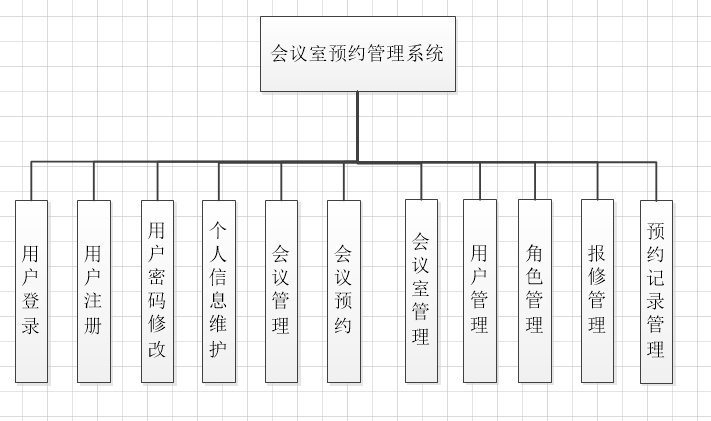
\includegraphics[width=0.85\textwidth]{figures/fig3-1.png}
  \caption{系统功能图}
  \label{fig:3-1}
\end{figure}

\subsection{角色分析}
在研究分析后，确定会议室预约管理系统的角色有普通用户及管理员。本系统的角色职责如表~\ref{tab:3-1}~所示：

\begin{table}[htbp]
  \centering
  \caption{角色职责表}
  \label{tab:3-1}
  \zihao{5}\songti
  \begin{tabular}{|c|p{11.5cm}|}
    \hline
    角色 & 操作 \\
    \hline
    普通用户 & 用户注册，登录系统，密码修改，个人信息维护，查看个人会议日程，会议预约、查询、编辑、删除等操作，查看会议室操作。 \\
    \hline
    管理员 & 对用户信息进行增、删、改、查等操作，对会议室信息进行增、删、改、查等操作，对预约记录进行查询、导出等操作，对部门信息进行增、删、改、查等操作，对报修信息进行增、删、改、查等操作，对角色进行增、删、改、查等操作。 \\
    \hline
  \end{tabular}
\end{table}

\subsection{角色功能分析}
以下给出本系统的总用例图，此图中包括用户注册、登录、查询会议室、密码修改、个人信息维护、查看会议日程、会议预约、会议管理以及管理员对报修的管理、对会议室的管理、对用户的管理、对角色的管理、对预约记录的管理等用例。如图~\ref{fig:3-2}~所示：

\begin{figure}[htbp]
  \centering
  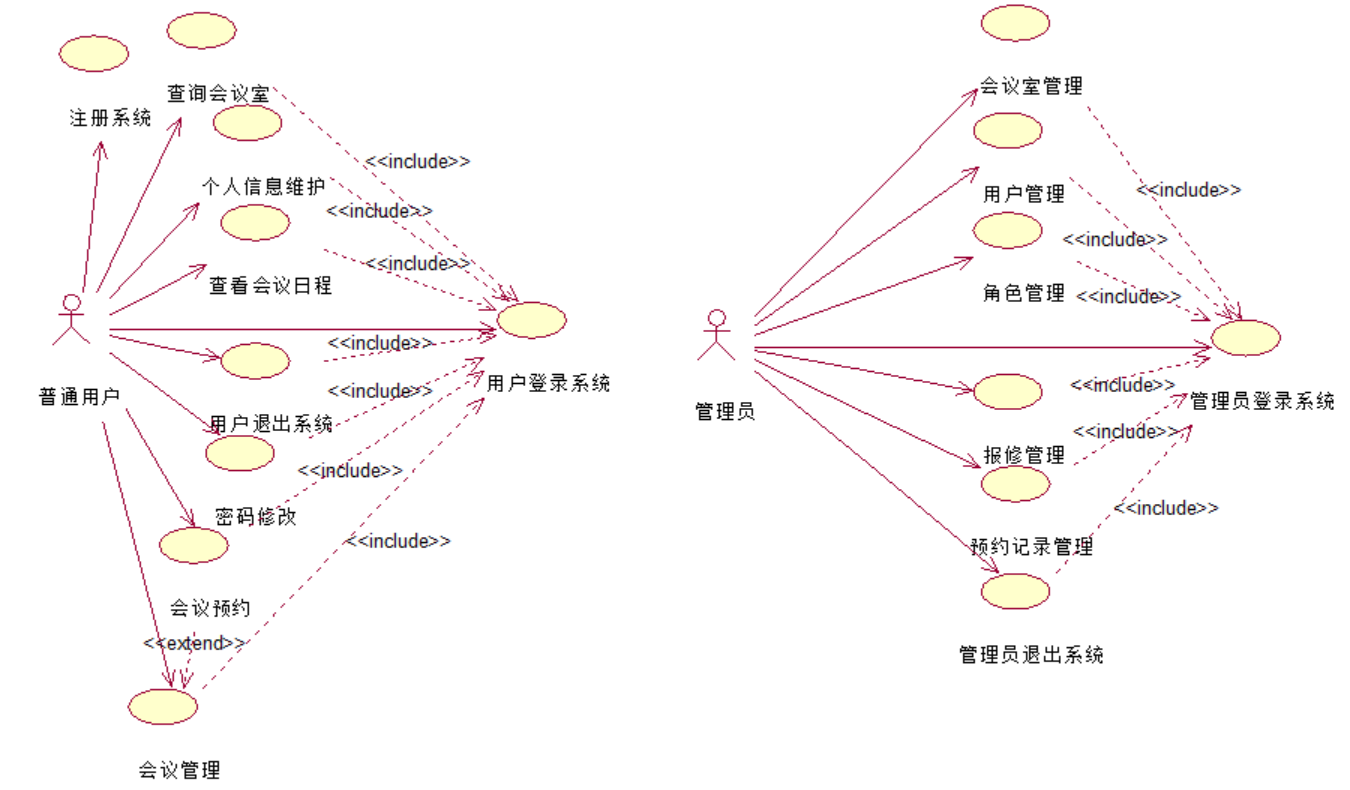
\includegraphics[width=0.95\textwidth]{figures/fig3-2.png}
  \caption{会议室预约管理系统用例图}
  \label{fig:3-2}
\end{figure}

\section{用例建模}
用例是通过用户的使用场景来获取需求的技术，用其来说明是谁要使用系统，以及系统可以提供给他们的功能。而用例图则体现了用户与用户、功能与功能之间的关系，描述了系统拥有的所有用户以及每种用户可以使用的功能。

本系统的典型用例如下：

\subsection{登录模块用例图}
登录模块用例如图~\ref{fig:3-3}~所示，用例描述如表~\ref{tab:3-2}~所示：

\begin{figure}[htbp]
  \centering
  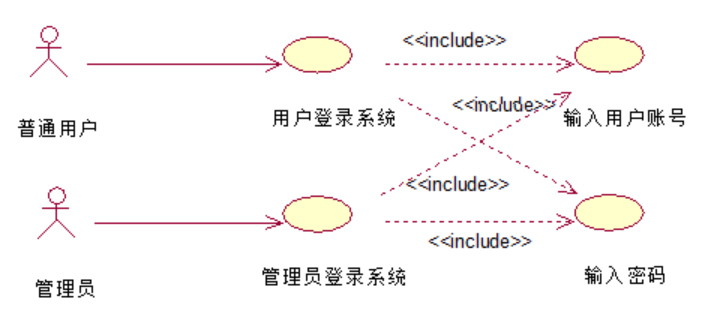
\includegraphics[width=0.55\textwidth]{figures/fig3-3.png}
  \caption{登录模块用例图}
  \label{fig:3-3}
\end{figure}

\begin{table}[htbp]
  \centering
  \caption{登录模块用例描述}
  \label{tab:3-2}
  \zihao{5}\songti
  \begin{tabular}{|c|p{11.5cm}|}
    \hline
    项目 & 说明 \\
    \hline
    用例 & 登录模块 \\
    \hline
    描述 & 用户填写相关信息，系统验证，如果正确则登录成功，否则登录失败。 \\
    \hline
    参与者 & 普通用户、管理员 \\
    \hline
    前置条件 & 用户已成功注册。 \\
    \hline
    后置条件 & 用户根据不同的角色权限可以使用相对应的功能。 \\
    \hline
    基本事件流 & 1、 用户进入本系统登录页面；\newline 2、 用户输入账号等相关信息，点击确认；\newline 3、 系统验证用户信息，验证通过，跳转至系统首页，若信息错误，系统显示提示，并转向基本流 1。 \\
    \hline
    备选事件流 & 1、 用户要求放弃会议室预约管理系统的登录。\newline 2、 用户输入信息有误，系统提示错误。 \\
    \hline
  \end{tabular}
\end{table}

\subsection{注册系统用例图}
注册系统用例如图~\ref{fig:3-4}~所示，用例描述如表~\ref{tab:3-3}~所示：

\begin{figure}[htbp]
  \centering
  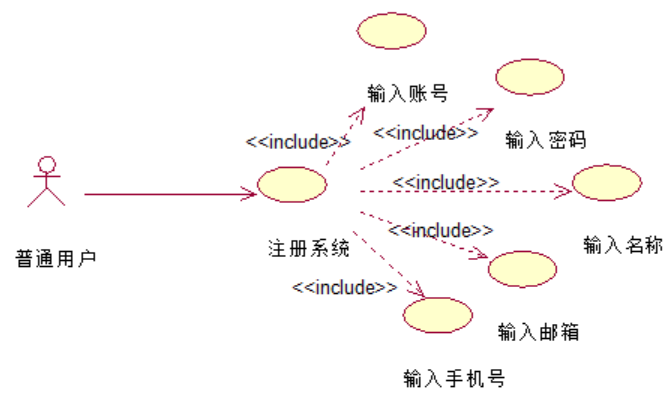
\includegraphics[width=0.55\textwidth]{figures/fig3-4.png}
  \caption{注册系统用例图}
  \label{fig:3-4}
\end{figure}

\begin{table}[htbp]
  \centering
  \caption{注册系统用例描述}
  \label{tab:3-3}
  \zihao{5}\songti
  \begin{tabular}{|c|p{11.5cm}|}
    \hline
    项目 & 说明 \\
    \hline
    用例 & 注册系统 \\
    \hline
    描述 & 用户要使用本系统提供的功能，需要先注册一个账号。 \\
    \hline
    参与者 & 普通用户 \\
    \hline
    前置条件 & 未注册过本系统的用户。 \\
    \hline
    后置条件 & 用户成功注册。 \\
    \hline
    基本事件流 & 1、用户进入本系统注册页面；\newline 2、系统显示注册界面；\newline 3、用户输入账号、密码、名称等必填信息并确认；\newline 4、系统验证信息是否输入正确，如果错误，系统显示信息，并转向基本流 3，如果正确，跳转至登录页面。 \\
    \hline
    备选事件流 & 1、 账号已被注册，系统显示提示信息。\newline 2、 邮箱、手机号重复注册使用，系统显示提示信息。\newline 3、 名称已被注册，系统显示提示信息。 \\
    \hline
  \end{tabular}
\end{table}

\subsection{退出登录模块用例}
退出登录模块用例如图~\ref{fig:3-5}~所示，用例描述如表~\ref{tab:3-4}~所示：

\begin{figure}[htbp]
  \centering
  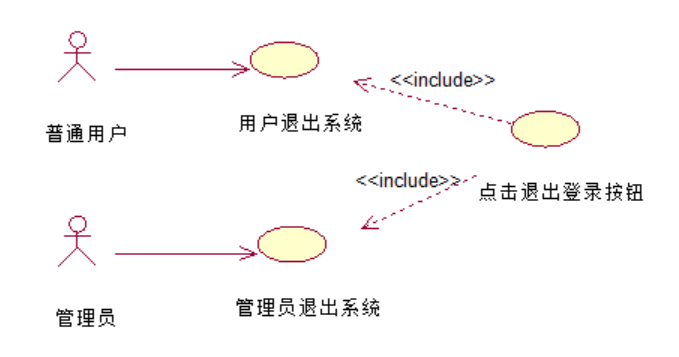
\includegraphics[width=0.55\textwidth]{figures/fig3-5.png}
  \caption{退出登录模块用例图}
  \label{fig:3-5}
\end{figure}

\begin{table}[htbp]
  \centering
  \caption{退出登录模块用例描述}
  \label{tab:3-4}
  \zihao{5}\songti
  \begin{tabular}{|c|p{11.5cm}|}
    \hline
    项目 & 说明 \\
    \hline
    用例 & 退出登录模块 \\
    \hline
    描述 & 用户根据需要退出系统。 \\
    \hline
    参与者 & 普通用户、管理员 \\
    \hline
    前置条件 & 用户已成功登录系统。 \\
    \hline
    后置条件 & 成功退出系统。 \\
    \hline
    基本事件流 & 1、 普通用户或管理员点击退出登录按钮；\newline 2、 退出登录成功；\newline 3、 跳转至系统登录页面。 \\
    \hline
    备选事件流 & 无 \\
    \hline
  \end{tabular}
\end{table}

\subsection{个人信息维护用例}
个人信息维护用例如图~\ref{fig:3-6}~所示，用例描述如表~\ref{tab:3-5}~所示：

\begin{figure}[htbp]
  \centering
  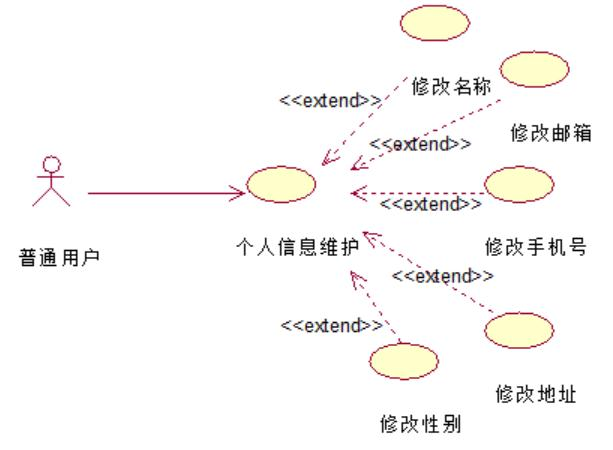
\includegraphics[width=0.55\textwidth]{figures/fig3-6.png}
  \caption{个人信息维护用例图}
  \label{fig:3-6}
\end{figure}

\begin{table}[htbp]
  \centering
  \caption{个人信息维护用例描述}
  \label{tab:3-5}
  \zihao{5}\songti
  \begin{tabular}{|c|p{11.5cm}|}
    \hline
    项目 & 说明 \\
    \hline
    用例 & 个人信息维护 \\
    \hline
    描述 & 用户可根据需要修改个人的信息。 \\
    \hline
    参与者 & 普通用户 \\
    \hline
    前置条件 & 用户成功登录系统。 \\
    \hline
    后置条件 & 系统保存个人信息。 \\
    \hline
    基本事件流 & 1、 用户成功登录系统并请求修改个人信息；\newline 2、 系统显示用户个人信息界面；\newline 3、 用户点击编辑按钮；\newline 4、 用户根据需要对信息修改，点击保存；\newline 5、 系统验证修改的信息，如果验证未通过，系统显示信息并转向基本流 3，如果验证通过，系统保存用户修改后的信息。 \\
    \hline
    备选事件流 & 1、 用户点击取消按钮，系统转向基本流 2。\newline 2、 用户不保存修改信息，系统转向基本流 2。 \\
    \hline
  \end{tabular}
\end{table}

\subsection{密码修改用例}
密码修改用例如图~\ref{fig:3-7}~所示，用例描述如表~\ref{tab:3-6}~所示：

\begin{figure}[htbp]
  \centering
  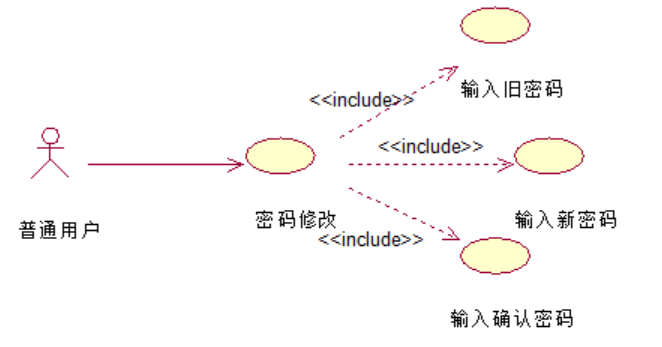
\includegraphics[width=0.55\textwidth]{figures/fig3-7.png}
  \caption{密码修改用例图}
  \label{fig:3-7}
\end{figure}

\begin{table}[htbp]
  \centering
  \caption{密码修改用例描述}
  \label{tab:3-6}
  \zihao{5}\songti
  \begin{tabular}{|c|p{11.5cm}|}
    \hline
    项目 & 说明 \\
    \hline
    用例 & 密码修改 \\
    \hline
    描述 & 用于修改个人密码。 \\
    \hline
    参与者 & 普通用户 \\
    \hline
    前置条件 & 1、用户成功登录系统。\newline 2、用户拥有修改个人密码权限。 \\
    \hline
    后置条件 & 系统保存个人密码。 \\
    \hline
    基本事件流 & 1、 用户成功登录系统并请求修改密码；\newline 2、 系统显示修改密码界面；\newline 3、 用户输入旧密码、新密码、确认密码，点击确认；\newline 4、 系统验证，如果验证未通过，系统显示信息并转向基本流 3，如果验证通过，系统保存用户修改。 \\
    \hline
    备选事件流 & 1、 用户点击取消按钮，系统转向基本流 2。\newline 2、 用户不保存修改密码，系统转向基本流 2。 \\
    \hline
  \end{tabular}
\end{table}

\subsection{会议管理用例}
会议管理用例如图~\ref{fig:3-8}~所示，用例描述如表~\ref{tab:3-7}~所示：

\begin{figure}[htbp]
  \centering
  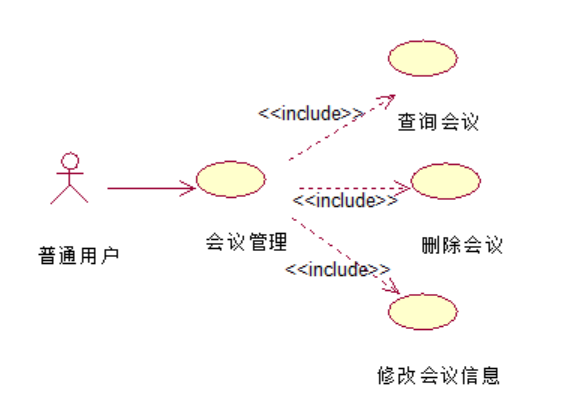
\includegraphics[width=0.55\textwidth]{figures/fig3-8.png}
  \caption{会议管理用例图}
  \label{fig:3-8}
\end{figure}

\begin{table}[htbp]
  \centering
  \caption{会议管理用例描述}
  \label{tab:3-7}
  \zihao{5}\songti
  \begin{tabular}{|c|p{11.5cm}|}
    \hline
    项目 & 说明 \\
    \hline
    用例 & 会议管理 \\
    \hline
    描述 & 用于管理个人会议。 \\
    \hline
    参与者 & 普通用户 \\
    \hline
    前置条件 & 1、用户成功登录系统。\newline 2、用户拥有会议管理权限。 \\
    \hline
    后置条件 & 系统保存信息。 \\
    \hline
    基本事件流 & 1、 用户成功登录系统并请求管理个人会议；\newline 2、 系统显示会议管理界面；\newline 3、 用户根据实际情况，对个人会议进行查询、删除、编辑等操作；\newline 4、 对会议的操作成功执行。 \\
    \hline
    备选事件流 & 1、 用户点击取消按钮，系统转向基本流 2。\newline 2、 用户不保存修改后的会议信息，系统转向基本流 2。 \\
    \hline
  \end{tabular}
\end{table}

\subsection{搜索查询会议室用例}
搜索查询会议室用例如图~\ref{fig:3-9}~所示，用例描述如表~\ref{tab:3-8}~所示：

\begin{figure}[htbp]
  \centering
  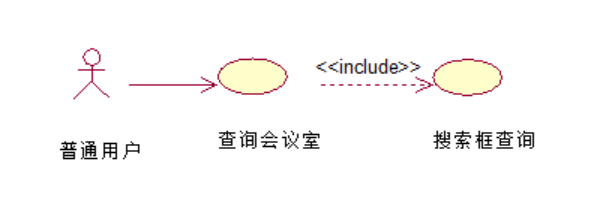
\includegraphics[width=0.55\textwidth]{figures/fig3-9.png}
  \caption{搜索查询会议室用例图}
  \label{fig:3-9}
\end{figure}

\begin{table}[htbp]
  \centering
  \caption{搜索查询会议室用例描述}
  \label{tab:3-8}
  \zihao{5}\songti
  \begin{tabular}{|c|p{11.5cm}|}
    \hline
    项目 & 说明 \\
    \hline
    用例 & 查询会议室 \\
    \hline
    描述 & 用于查询会议室信息。 \\
    \hline
    参与者 & 普通用户 \\
    \hline
    前置条件 & 1、 用户成功登录系统。\newline 2、 用户拥有查询会议室信息权限。 \\
    \hline
    后置条件 & 系统显示用户所查询会议室信息。 \\
    \hline
    基本事件流 & 1、 用户成功登录系统；\newline 2、 用户请求搜索查询会议室；\newline 3、 系统显示会议室管理界面；\newline 4、 用户根据实际情况，对会议室进行查询操作；\newline 5、 系统显示会议室相关信息。 \\
    \hline
    备选事件流 & 用户搜索的会议室不存在，系统显示提示信息。 \\
    \hline
  \end{tabular}
\end{table}

\subsection{会议预约用例}
会议预约用例如图~\ref{fig:3-10}~所示，用例描述如表~\ref{tab:3-9}~所示：

\begin{figure}[htbp]
  \centering
  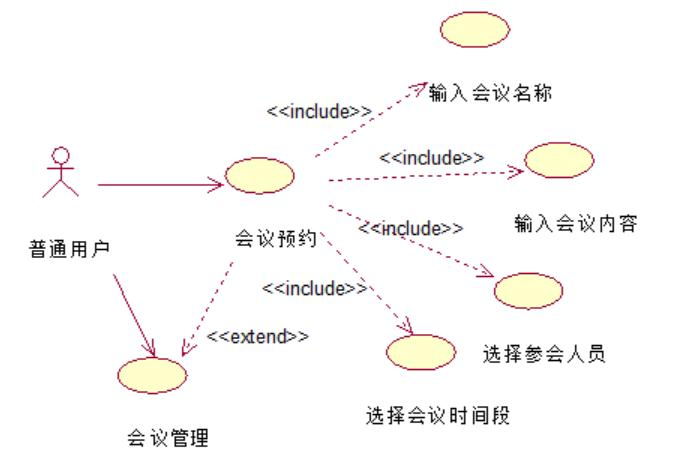
\includegraphics[width=0.55\textwidth]{figures/fig3-10.png}
  \caption{会议预约用例图}
  \label{fig:3-10}
\end{figure}

\begin{table}[htbp]
  \centering
  \caption{会议预约用例描述}
  \label{tab:3-9}
  \zihao{5}\songti
  \begin{tabular}{|c|p{11.5cm}|}
    \hline
    项目 & 说明 \\
    \hline
    用例 & 会议预约 \\
    \hline
    描述 & 用于预约会议。 \\
    \hline
    参与者 & 普通用户 \\
    \hline
    前置条件 & 1、 用户成功登录系统。\newline 2、 用户拥有预约会议权限。 \\
    \hline
    后置条件 & 系统保存预约会议信息。 \\
    \hline
    基本事件流 & 1、 用户成功登录系统并点击会议管理按钮；\newline 2、 系统显示会议管理界面；\newline 3、 用户点击创建会议按钮；\newline 4、 系统显示预约会议界面；\newline 5、 用户输入信息，点击保存；\newline 6、 系统保存信息。 \\
    \hline
    备选事件流 & 1、 如果用户所预约会议时间小于当前时间，系统显示提示信息，并转向基本流 3。\newline 2、 如果用户一个会议选择多个时间段，系统显示提示信息，并转向基本流 3。\newline 3、 如果用户有必填信息未填写时点击保存按钮，系统显示提示信息，并转向基本流 3。\newline 4、 用户点击取消按钮，系统转向基本流 2。\newline 5、 用户不保存预约会议信息，系统转向基本流 2。 \\
    \hline
  \end{tabular}
\end{table}

\subsection{会议室管理用例}
会议室管理用例如图~\ref{fig:3-11}~所示，用例描述如表~\ref{tab:3-10}~所示：

\begin{figure}[htbp]
  \centering
  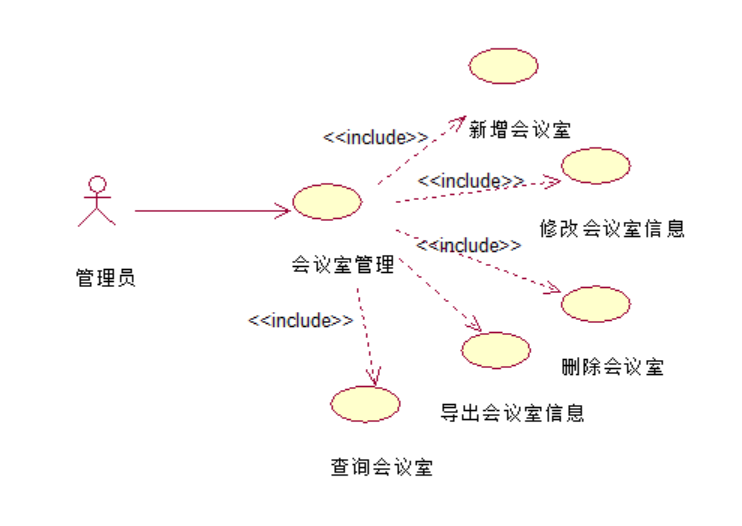
\includegraphics[width=0.55\textwidth]{figures/fig3-11.png}
  \caption{会议室管理用例图}
  \label{fig:3-11}
\end{figure}

\begin{table}[htbp]
  \centering
  \caption{会议室管理用例描述}
  \label{tab:3-10}
  \zihao{5}\songti
  \begin{tabular}{|c|p{11.5cm}|}
    \hline
    项目 & 说明 \\
    \hline
    用例 & 会议室管理 \\
    \hline
    描述 & 用于管理会议室信息。 \\
    \hline
    参与者 & 管理员 \\
    \hline
    前置条件 & 管理员成功登录系统，点击会议室管理。 \\
    \hline
    后置条件 & 系统保存会议室数据。 \\
    \hline
    基本事件流 & 1、 管理员成功登录系统；\newline 2、 系统显示会议室管理界面；\newline 3、 管理员对会议室进行所需要的操作；\newline 4、 对会议室的操作成功执行。 \\
    \hline
    备选事件流 & 1、 管理员点击取消按钮，系统转向基本流 2。\newline 2、 管理员不保存新增或修改后的会议室信息，系统转向基本流 2。 \\
    \hline
  \end{tabular}
\end{table}

\subsection{用户管理用例}
用户管理用例如图~\ref{fig:3-12}~所示，用例描述如表~\ref{tab:3-11}~所示：

\begin{figure}[htbp]
  \centering
  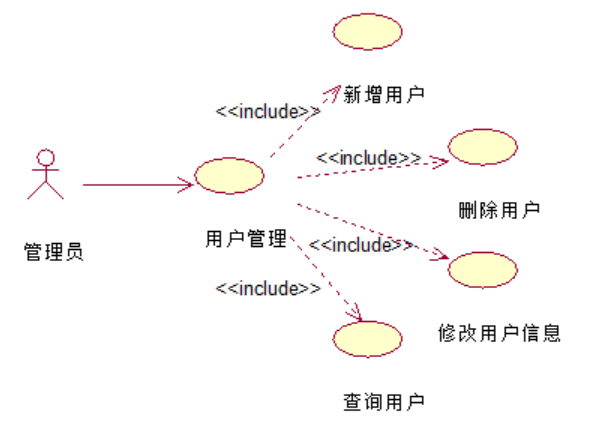
\includegraphics[width=0.55\textwidth]{figures/fig3-12.png}
  \caption{用户管理用例图}
  \label{fig:3-12}
\end{figure}

\begin{table}[htbp]
  \centering
  \caption{用户管理用例描述}
  \label{tab:3-11}
  \zihao{5}\songti
  \begin{tabular}{|c|p{11.5cm}|}
    \hline
    项目 & 说明 \\
    \hline
    用例 & 用户管理 \\
    \hline
    描述 & 用于管理系统用户信息。 \\
    \hline
    参与者 & 管理员 \\
    \hline
    前置条件 & 1、 管理员成功登录系统。\newline 2、 点击用户管理。 \\
    \hline
    后置条件 & 系统保存用户数据。 \\
    \hline
    基本事件流 & 1、 管理员成功登录系统；\newline 2、 系统显示用户管理界面；\newline 3、 管理员对用户信息进行所需要的操作；\newline 4、 操作成功执行。 \\
    \hline
    备选事件流 & 1、 管理员点击取消按钮，系统转向基本流 2。\newline 2、 管理员不保存新增或修改后的用户信息，系统转向基本流 2。 \\
    \hline
  \end{tabular}
\end{table}

\subsection{角色管理用例}
角色管理用例如图~\ref{fig:3-13}~所示，用例描述如表~\ref{tab:3-12}~所示：

\begin{figure}[htbp]
  \centering
  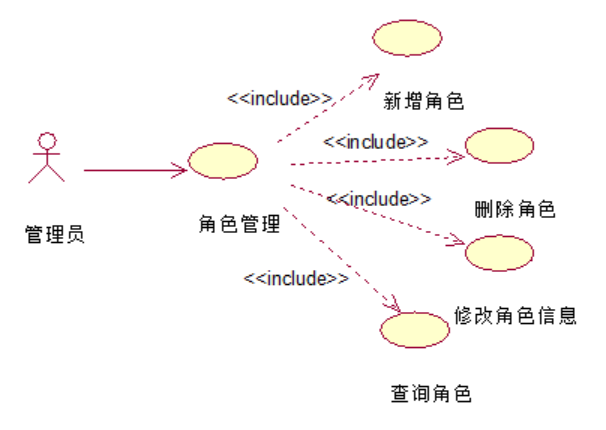
\includegraphics[width=0.55\textwidth]{figures/fig3-13.png}
  \caption{角色管理用例图}
  \label{fig:3-13}
\end{figure}

\begin{table}[htbp]
  \centering
  \caption{角色管理用例描述}
  \label{tab:3-12}
  \zihao{5}\songti
  \begin{tabular}{|c|p{11.5cm}|}
    \hline
    项目 & 说明 \\
    \hline
    用例 & 角色管理 \\
    \hline
    描述 & 用于管理角色信息。 \\
    \hline
    参与者 & 管理员 \\
    \hline
    前置条件 & 1、 管理员成功登录系统。\newline 2、 点击角色管理。 \\
    \hline
    后置条件 & 系统保存角色数据。 \\
    \hline
    基本事件流 & 1、 管理员成功登录系统并点击角色管理按钮；\newline 2、 系统显示角色管理界面；\newline 3、 管理员对角色信息进行所需要的操作；\newline 4、 对角色的操作成功执行。 \\
    \hline
    备选事件流 & 1、 管理员点击取消按钮，系统转向基本流 2。\newline 2、 管理员不保存新增或修改后的角色信息，系统转向基本流 2。 \\
    \hline
  \end{tabular}
\end{table}

\subsection{报修管理用例}
报修管理用例如图~\ref{fig:3-14}~所示，用例描述如表~\ref{tab:3-13}~所示：

\begin{figure}[htbp]
  \centering
  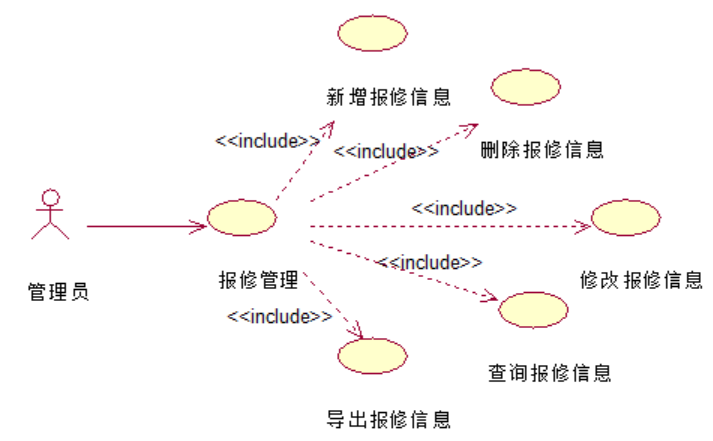
\includegraphics[width=0.55\textwidth]{figures/fig3-14.png}
  \caption{报修管理用例图}
  \label{fig:3-14}
\end{figure}

\begin{table}[htbp]
  \centering
  \caption{报修管理用例描述}
  \label{tab:3-13}
  \zihao{5}\songti
  \begin{tabular}{|c|p{11.5cm}|}
    \hline
    项目 & 说明 \\
    \hline
    用例 & 报修管理 \\
    \hline
    描述 & 用于管理会议室报修信息。 \\
    \hline
    参与者 & 管理员 \\
    \hline
    前置条件 & 1、 管理员成功登录系统。\newline 2、 点击报修管理。 \\
    \hline
    后置条件 & 系统保存报修数据。 \\
    \hline
    基本事件流 & 1、 管理员成功登录系统并点击报修管理按钮；\newline 2、 系统显示报修管理界面；\newline 3、 管理员根据实际情况，对报修信息进行所需要的操作；\newline 4、 对报修的操作成功执行。 \\
    \hline
    备选事件流 & 1、 管理员点击取消按钮，系统转向基本流 2。\newline 2、 管理员不保存新增或修改后的报修信息，系统转向基本流 2。 \\
    \hline
  \end{tabular}
\end{table}

\subsection{预约记录管理用例}
预约记录管理用例如图~\ref{fig:3-15}~所示，用例描述如表~\ref{tab:3-14}~所示：

\begin{figure}[htbp]
  \centering
  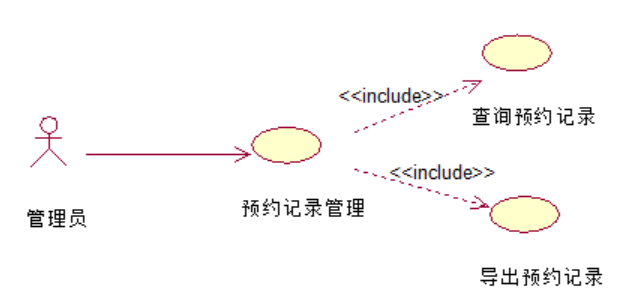
\includegraphics[width=0.55\textwidth]{figures/fig3-15.png}
  \caption{预约记录管理用例图}
  \label{fig:3-15}
\end{figure}

\begin{table}[htbp]
  \centering
  \caption{预约记录管理用例描述}
  \label{tab:3-14}
  \zihao{5}\songti
  \begin{tabular}{|c|p{11.5cm}|}
    \hline
    项目 & 说明 \\
    \hline
    用例 & 预约记录管理 \\
    \hline
    描述 & 用于管理预约记录信息。 \\
    \hline
    参与者 & 管理员 \\
    \hline
    前置条件 & 1、 管理员成功登录系统。\newline 2、 点击预约记录管理。 \\
    \hline
    后置条件 & 系统保存预约记录数据。 \\
    \hline
    基本事件流 & 1、 管理员成功登录系统并点击预约记录管理；\newline 2、 系统显示预约记录管理界面；\newline 3、 管理员根据实际情况，对预约记录信息进行所需要的操作；\newline 4、 对预约记录的操作成功执行。 \\
    \hline
    备选事件流 & 无 \\
    \hline
  \end{tabular}
\end{table}

\section{类图}
类图是定义其他图如活动图、顺序图的基础部分，是静态视图。类图描述了类、接口、协作以及它们之间的关系,从而简化了对系统的理解\cite{ref7}。

会议室预约管理系统的类图中普通用户的基本属性包括用户 ID、账号、名称、密码。其可以调用的类有登录系统、密码修改、退出登录、会议管理、注册、个人信息维护、搜索查询会议室、会议预约。管理员的基本属性包括用户名、密码、管理员 ID，管理员可以调用的类有登录系统、会议室管理、预约记录管理、报修管理、用户管理、退出系统、角色管理。本系统的类图如图~\ref{fig:3-16}~所示：

\begin{figure}[htbp]
  \centering
  \includegraphics[width=\textwidth]{figures/fig3-16.png}
  \caption{系统需求类图}
  \label{fig:3-16}
\end{figure}

\section{活动图}
UML 活动图本质上是一种流程图，描述了系统指定功能或任务所必须执行的活动流程\cite{ref8}，即用什么样的动作在何时以及何处来做什么。并且活动图支持并行活动。

本系统的典型活动图如下：

\subsection{普通用户登录模块活动图}
普通用户登录会议室预约管理系统步骤如下：

第一步：用户进入会议室预约管理系统登录界面；

第二步：按照提示填写登录信息并点击登录；

第三步：系统判断用户账号和密码是否正确；

第四步：系统验证信息，若正确，跳转至系统首页，否则验证失败，系统显示信息。

普通用户登录模块活动图如图~\ref{fig:3-17}~所示。

\begin{figure}[htbp]
  \centering
  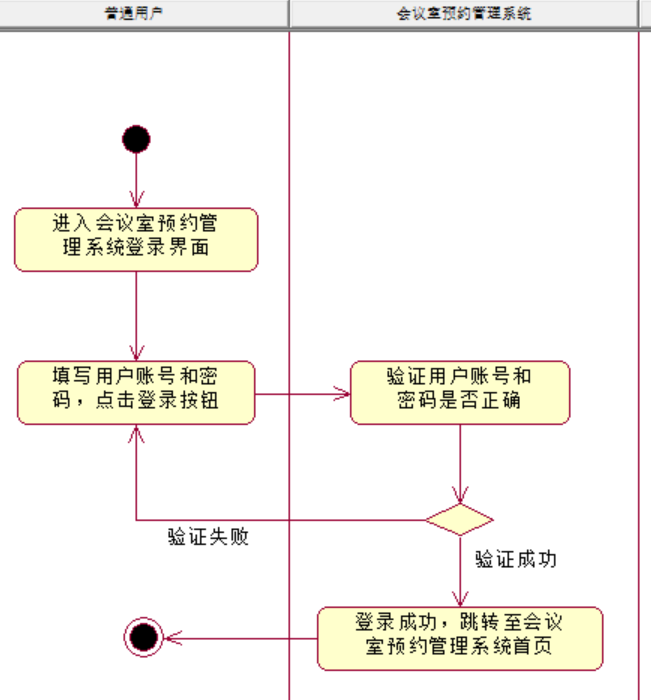
\includegraphics[width=0.5\textwidth]{figures/fig3-17.png}
  \caption{普通用户登录模块活动图}
  \label{fig:3-17}
\end{figure}

\subsection{普通用户注册模块活动图}
普通用户注册会议室预约管理系统步骤如下：

第一步：用户进入会议室预约管理系统注册界面；

第二步：按照提示填写用户账号、密码、名称、邮箱、手机号等信息并点击注册；

第三步：后台判断用户账号是否重复，如果重复返回第二步；

第四步：后台判断用户邮箱、手机号格式是否正确，如果不正确则返回第二步；

第五步：注册成功后，跳转至会议室预约管理系统登录界面。

普通用户注册模块活动图如图~\ref{fig:3-18}~所示。

\begin{figure}[htbp]
  \centering
  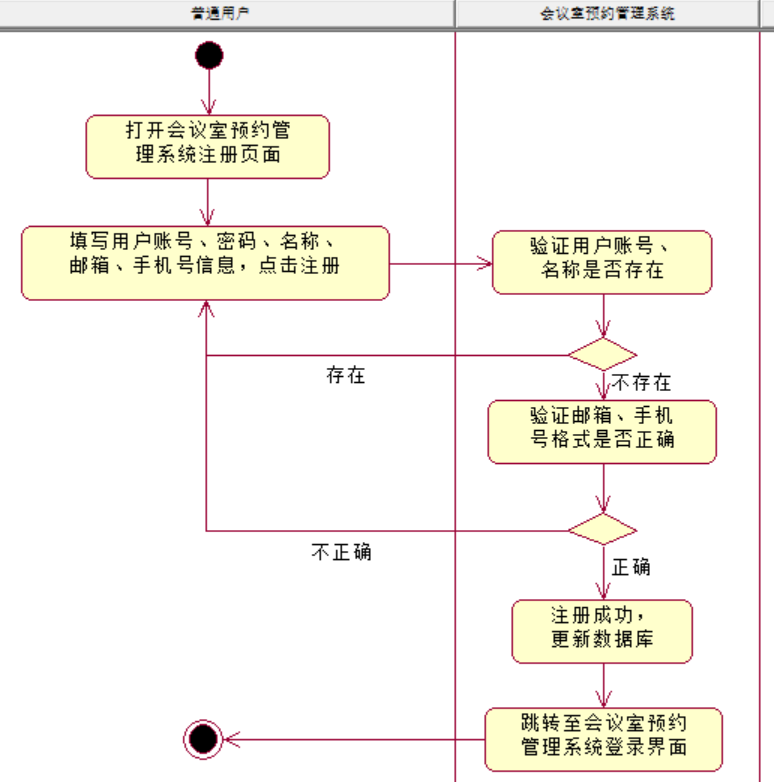
\includegraphics[width=0.5\textwidth]{figures/fig3-18.png}
  \caption{普通用户注册模块活动图}
  \label{fig:3-18}
\end{figure}

\subsection{普通用户密码修改活动图}
普通用户修改密码步骤如下：

第一步：用户成功登录会议室预约管理系统，并进入系统首页；

第二步：点击修改密码，跳转至密码修改界面；

第三步：输入旧密码、新密码及确认密码，点击确认修改；

第四步：后台判断用户旧密码是否正确，如果错误则返回第三步；

第五步：后台判断用户两次密码输入是否一致，如果不一致则返回第三步；

第六步：系统提示密码修改成功。

普通用户密码修改活动图如图~\ref{fig:3-19}~所示。

\begin{figure}[htbp]
  \centering
  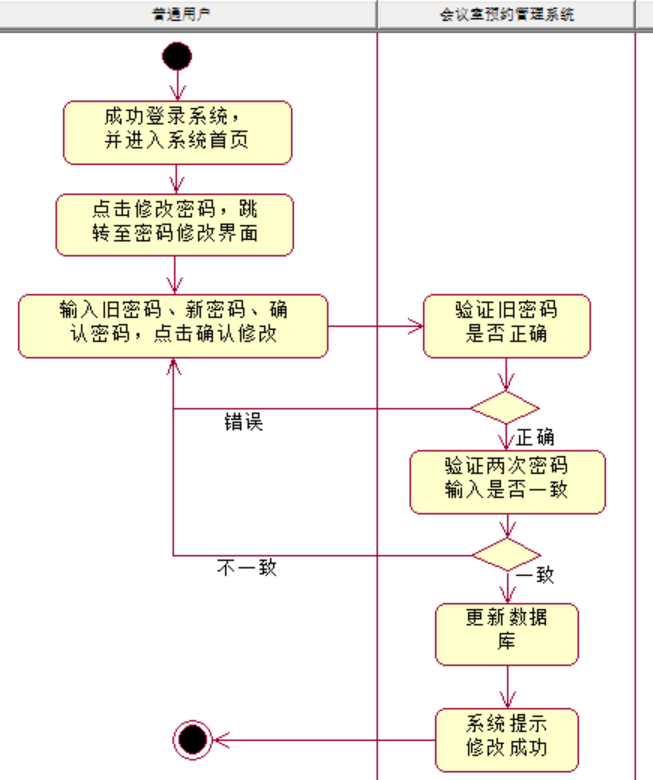
\includegraphics[width=0.5\textwidth]{figures/fig3-19.png}
  \caption{普通用户密码修改活动图}
  \label{fig:3-19}
\end{figure}

\subsection{普通用户个人信息维护活动图}
普通用户个人信息维护步骤如下：

第一步：用户成功登录会议室预约管理系统，并进入系统首页；

第二步：点击个人信息按钮，跳转至个人信息界面，点击编辑按钮；

第三步：根据需求修改名称、邮箱、手机号、地址与性别，并点击保存；

第四步：后台修改用户个人信息，并提示用户修改成功。

普通用户个人信息维护活动图如图~\ref{fig:3-20}~所示。

\begin{figure}[htbp]
  \centering
  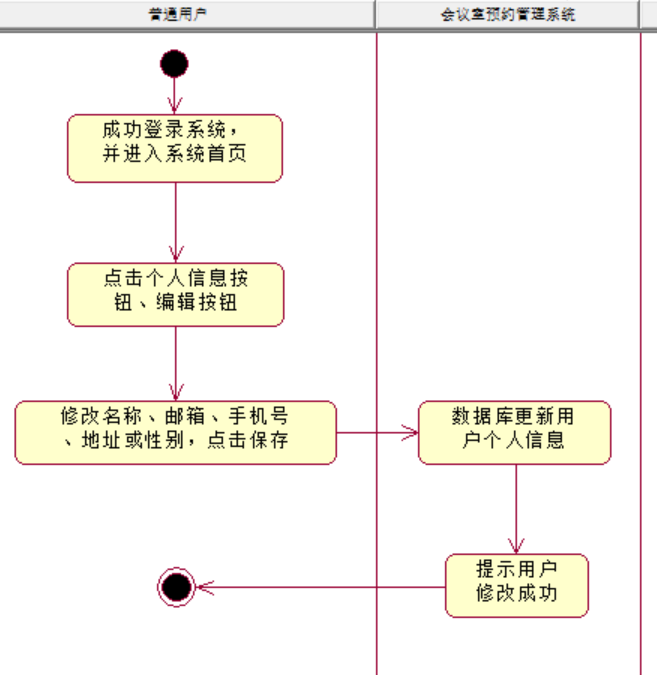
\includegraphics[width=0.5\textwidth]{figures/fig3-20.png}
  \caption{普通用户个人信息维护活动图}
  \label{fig:3-20}
\end{figure}

\subsection{普通用户会议预约活动图}
普通用户会议预约步骤如下：

第一步：用户成功登录会议室预约管理系统；

第二步：进入会议管理界面，点击创建会议，跳转至会议预约界面；

第三步：输入会议名称、内容，选择参会人员，选择相应会议室的预约时间段；

第四步：如果预约时间小于当前时间，系统提示用户，用户重新选择时间；

第五步：如果用户同一个会议预约两个时间段，系统提示用户；

第六步：点击保存按钮，系统提示用户保存成功，显示会议详情。

普通用户会议预约活动图如图~\ref{fig:3-21}~所示。

\begin{figure}[htbp]
  \centering
  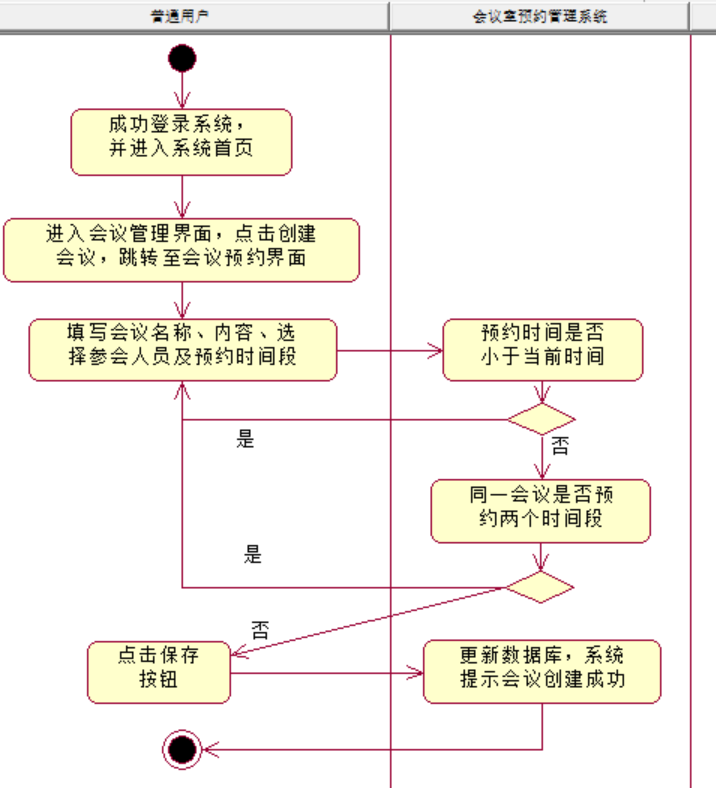
\includegraphics[width=0.5\textwidth]{figures/fig3-21.png}
  \caption{普通用户会议预约活动图}
  \label{fig:3-21}
\end{figure}

\subsection{预约记录查询活动图}
管理员查询预约记录步骤如下：

第一步：管理员登录系统进入首页；

第二步：进入预约记录管理界面，按照会议内容等查询预约记录信息；

第三步：后台筛选符合查询条件的预约记录数据，界面显示数据信息；

第四步：管理员查看预约记录信息。

预约记录查询活动图如图~\ref{fig:3-22}~所示。

\begin{figure}[htbp]
  \centering
  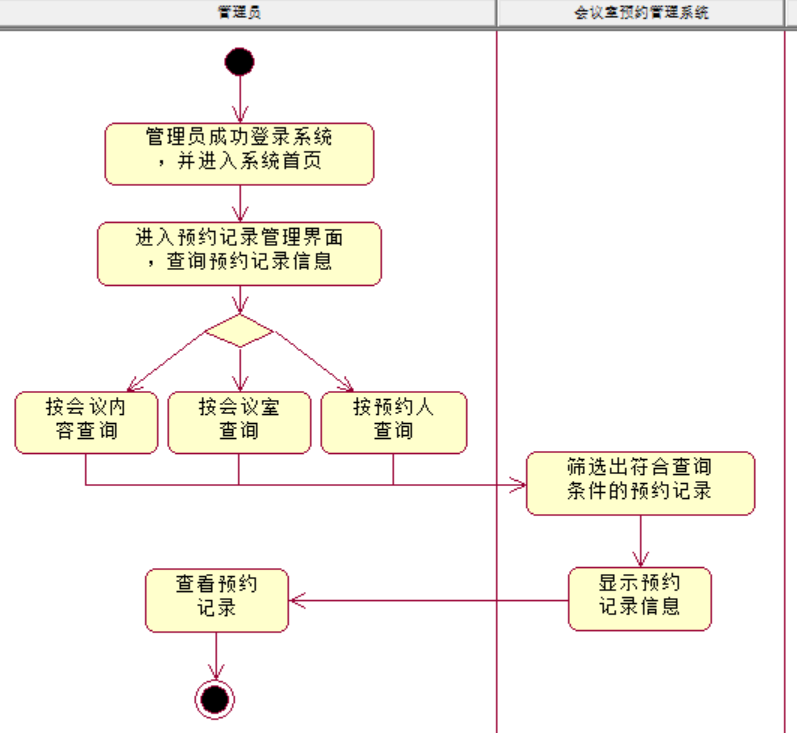
\includegraphics[width=0.55\textwidth]{figures/fig3-22.png}
  \caption{预约记录查询活动图}
  \label{fig:3-22}
\end{figure}

\subsection{报修新增模块活动图}
管理员新增报修记录步骤如下：

第一步：管理员登录系统进入首页；

第二步：进入报修管理界面，点击创建按钮；

第三步：选择会议室与报修人，填写报修内容，并点击保存按钮；

第四步：系统提示成功新增报修记录。

报修新增模块活动图如图~\ref{fig:3-23}~所示。

\begin{figure}[htbp]
  \centering
  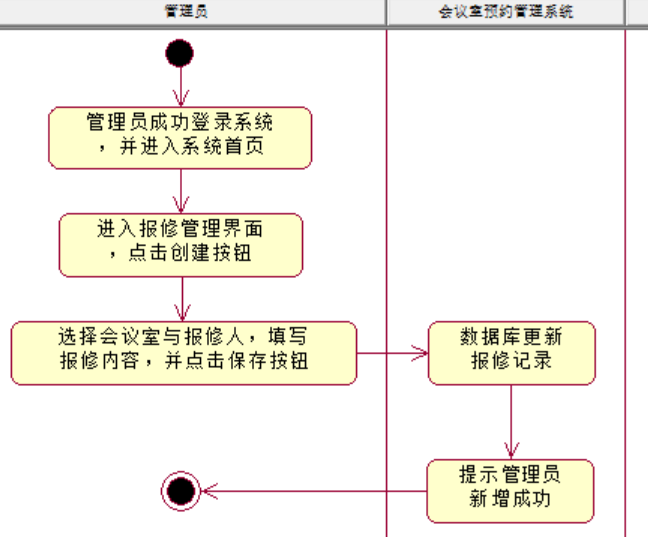
\includegraphics[width=0.5\textwidth]{figures/fig3-23.png}
  \caption{报修新增模块活动图}
  \label{fig:3-23}
\end{figure}

\subsection{用户信息修改模块活动图}
管理员修改用户信息模块步骤如下：

第一步：管理员登录系统进入首页；

第二步：进入用户管理界面，点击编辑，跳转至用户信息编辑界面；

第三步：管理员根据需求对用户信息进行修改，并点击确定按钮；

第四步：后台修改数据库中的信息，修改成功后提示管理员。

用户信息修改模块活动图如图~\ref{fig:3-24}~所示。

\begin{figure}[htbp]
  \centering
  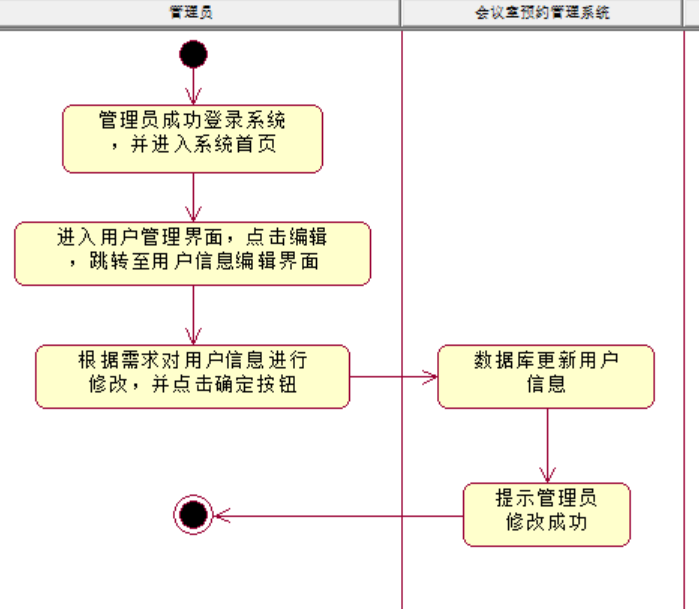
\includegraphics[width=0.5\textwidth]{figures/fig3-24.png}
  \caption{用户信息修改活动图}
  \label{fig:3-24}
\end{figure}

\chapter{系统设计}

在会议室预约管理系统的需求分析结束之后，需要进行系统设计。此阶段包括总体设计、类图设计、功能模块设计、组件图、部署图以及数据库设计。

\section{总体设计}
会议室预约管理系统包括用户登录、退出、注册模块、会议预约模块、用户密码修改、个人信息维护模块、报修管理模块、用户管理模块、角色管理模块、预约记录管理模块、会议室管理模块、会议管理模块。本系统总包图如图~\ref{fig:4-1}~所示：

\begin{figure}[htbp]
  \centering
  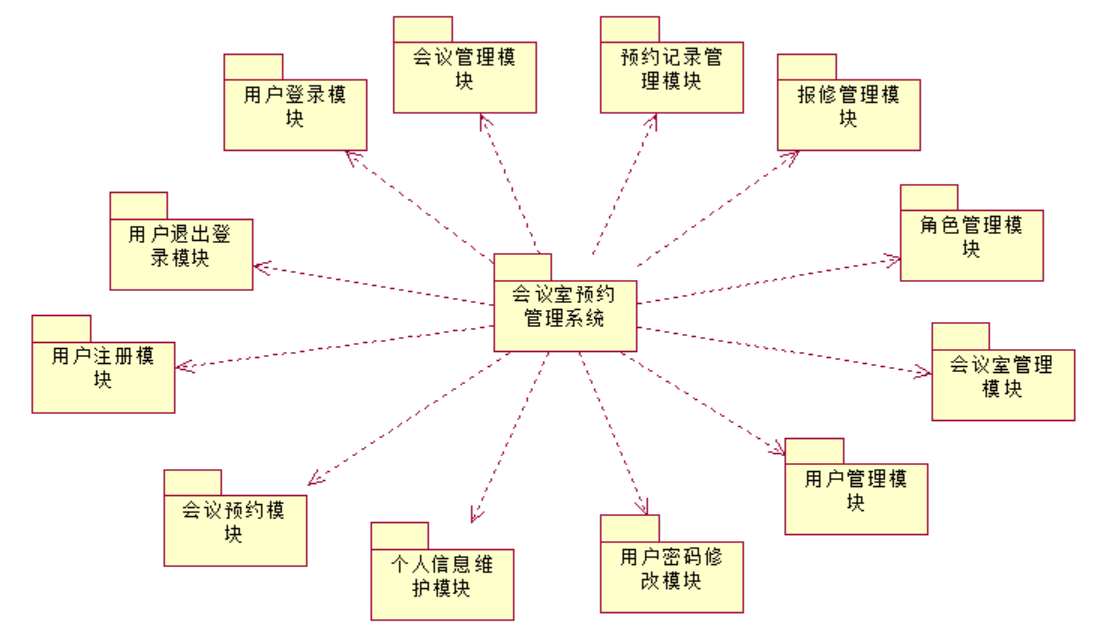
\includegraphics[width=0.9\textwidth]{figures/fig4-1.png}
  \caption{系统总包图}
  \label{fig:4-1}
\end{figure}

\section{类图设计}
根据系统需求分析，对会议室预约管理系统的各个类之间的关系设计类图，如图~\ref{fig:4-2}~所示：

\begin{figure}[htbp]
  \centering
  \includegraphics[width=0.95\textwidth,height=0.78\textheight,keepaspectratio]{figures/fig4-2.png}
  \caption{系统设计类图}
  \label{fig:4-2}
\end{figure}

\section{功能模块设计}
\subsection{登录模块顺序图设计}
控制层 AccountController 类中的方法调用相应的 Service 接口，再调用 Dao 层与数据库交互，获取登录账号 ID 以及角色，从而进入系统拥有相应的功能。登录模块顺序图如图~\ref{fig:4-3}~所示。

\begin{figure}[htbp]
  \centering
  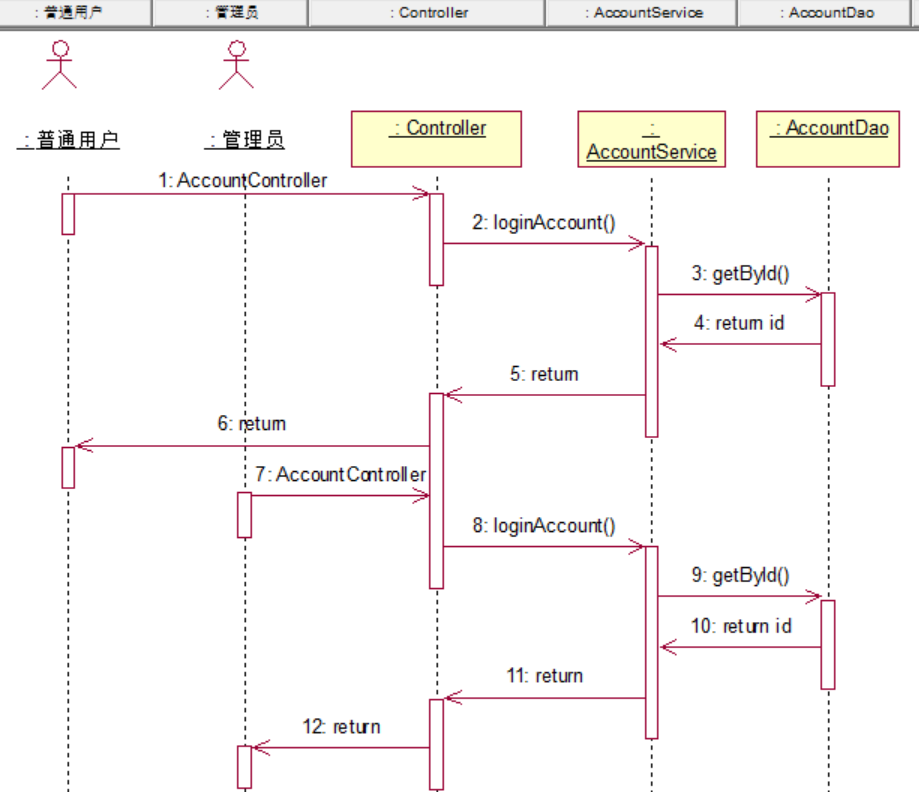
\includegraphics[width=0.9\textwidth,height=0.7\textheight,keepaspectratio]{figures/fig4-3.png}
  \caption{登录模块顺序图}
  \label{fig:4-3}
\end{figure}

\subsection{注册模块顺序图设计}
控制层 AccountController 类通过 createAccount 方法调用 Service 接口，根据条件查询数据库中是否有重复的信息，无重复则调用新增接口插入数据。注册模块顺序图如图~\ref{fig:4-4}~所示。

\begin{figure}[htbp]
  \centering
  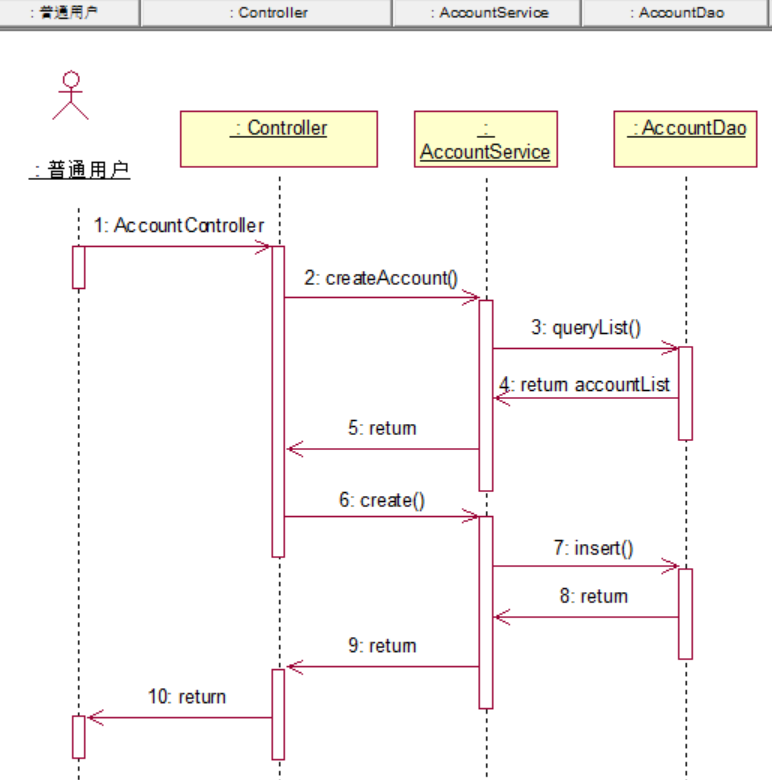
\includegraphics[width=0.9\textwidth,height=0.7\textheight,keepaspectratio]{figures/fig4-4.png}
  \caption{注册模块顺序图}
  \label{fig:4-4}
\end{figure}

\subsection{个人信息维护模块顺序图设计}
用户进入个人信息界面，系统调用 RoomController 类中的查询接口，界面显示个人信息。用户在保存修改操作时，调用此类中的修改接口，Service 层进行业务逻辑处理，再通过调用 Dao 层与数据库交互，根据原路径，将信息显示到界面。个人信息维护模块顺序图如图~\ref{fig:4-5}~所示。

\begin{figure}[htbp]
  \centering
  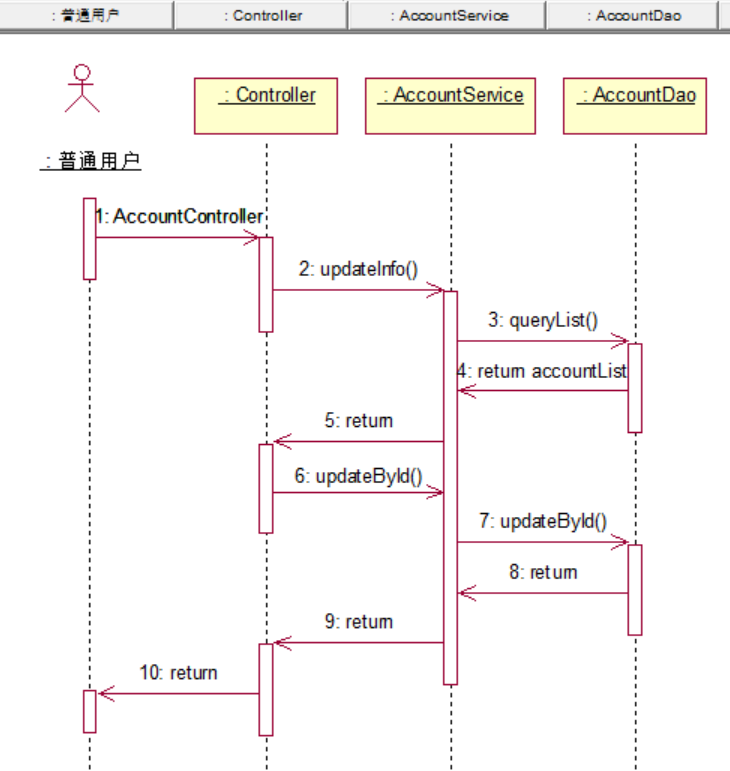
\includegraphics[width=0.9\textwidth,height=0.7\textheight,keepaspectratio]{figures/fig4-5.png}
  \caption{个人信息维护模块顺序图}
  \label{fig:4-5}
\end{figure}

\subsection{密码修改模块顺序图设计}
用户进行密码修改时，调用修改密码接口，获取当前登录账号信息，旧密码匹配成功且新密码格式正确，即可通过调用 Dao 层与数据库交互，根据原路径，将信息显示到界面。密码修改模块顺序图如图~\ref{fig:4-6}~所示。

\begin{figure}[htbp]
  \centering
  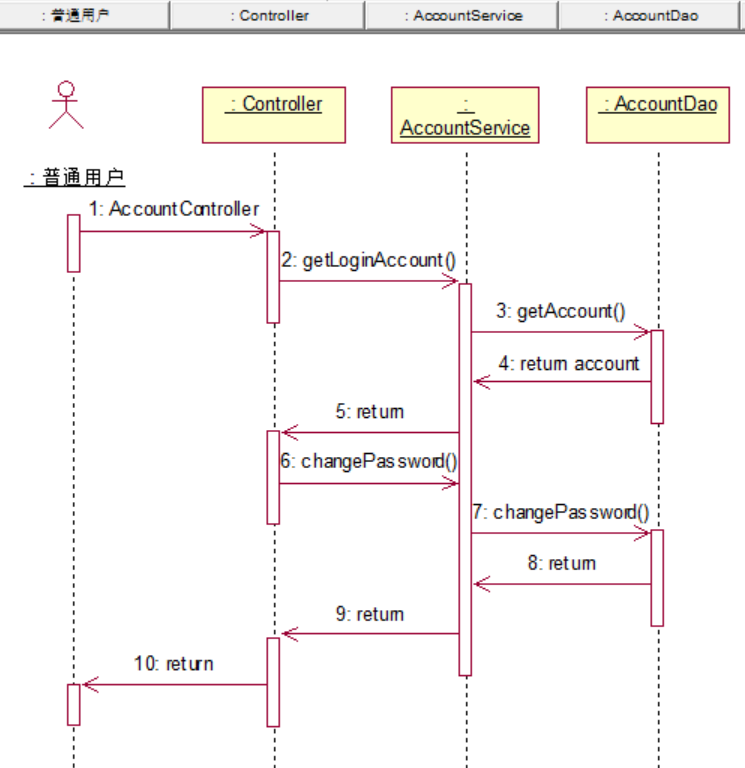
\includegraphics[width=0.9\textwidth,height=0.7\textheight,keepaspectratio]{figures/fig4-6.png}
  \caption{密码修改模块顺序图}
  \label{fig:4-6}
\end{figure}

\subsection{搜索查询会议室模块顺序图设计}
控制层 RoomController 类调用查询接口，Service 层进行业务逻辑处理，再通过调用 RoomDao 层与数据库进行交互，将信息按原路径，返回界面。搜索查询会议室模块顺序图如图~\ref{fig:4-7}~所示。

\begin{figure}[htbp]
  \centering
  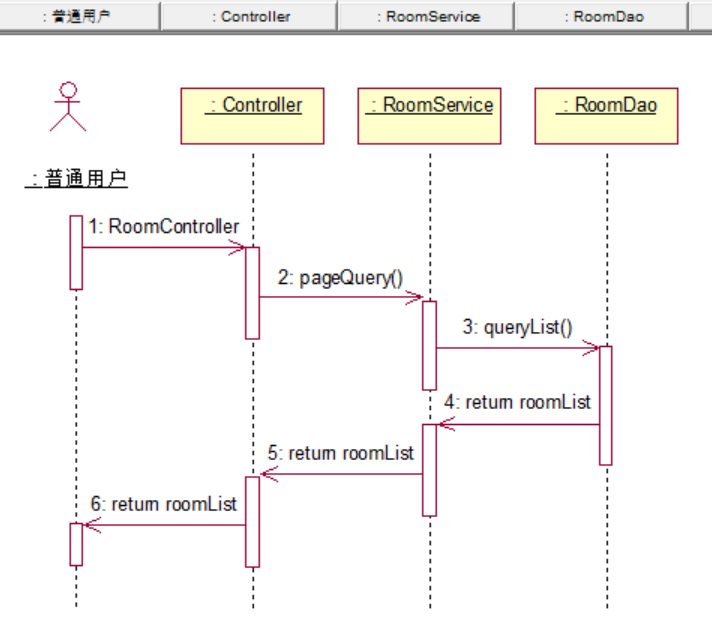
\includegraphics[width=0.9\textwidth,height=0.7\textheight,keepaspectratio]{figures/fig4-7.png}
  \caption{搜索查询会议室模块顺序图}
  \label{fig:4-7}
\end{figure}

\subsection{会议预约模块顺序图设计}
控制层 MeetingController 类调用新增接口，Service 层进行业务逻辑处理，再通过调用 ReserveDao 层与数据库进行交互，将信息按原路径，返回界面。会议预约模块顺序图如图~\ref{fig:4-8}~所示。

\begin{figure}[htbp]
  \centering
  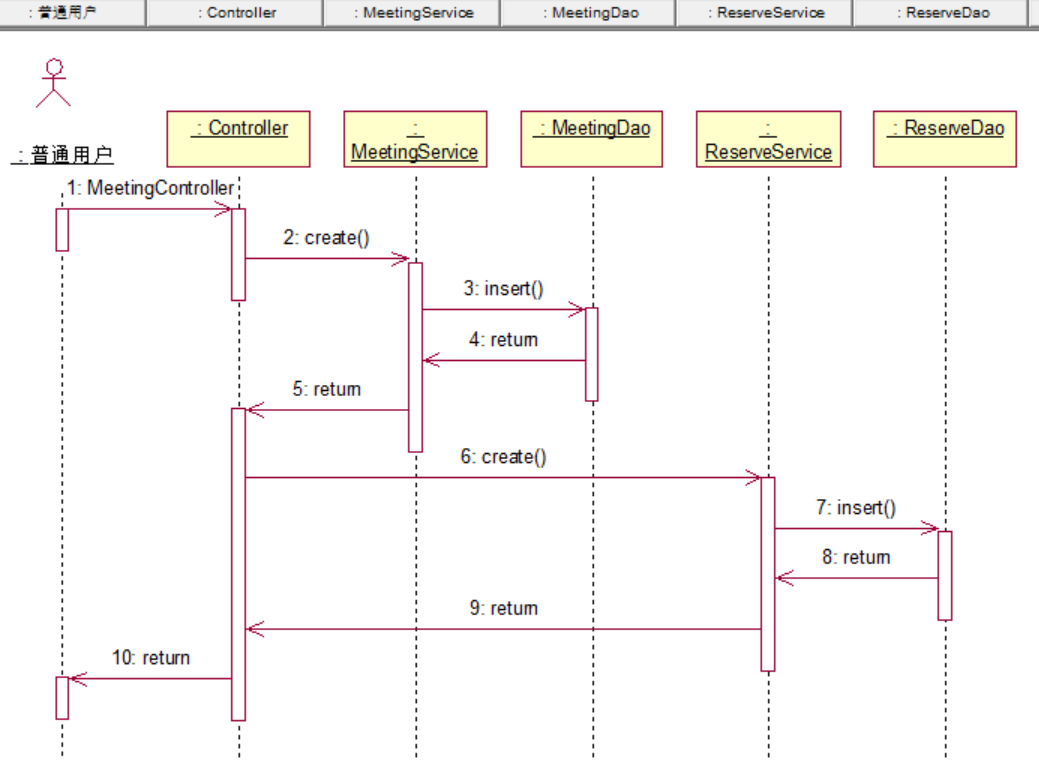
\includegraphics[width=0.9\textwidth,height=0.7\textheight,keepaspectratio]{figures/fig4-8.png}
  \caption{会议预约模块顺序图}
  \label{fig:4-8}
\end{figure}

\subsection{会议管理模块顺序图设计}
用户进入会议室管理界面，系统调用 MeetingController 类中的查询接口，界面显示会议信息。用户在进行其他操作时，调用此类中的相应接口，Service 层进行业务逻辑处理，再通过调用 Dao 层与数据库交互，根据原路径，将信息显示到界面。会议管理模块顺序图如图~\ref{fig:4-9}~所示。

\begin{figure}[htbp]
  \centering
  \includegraphics[width=0.9\textwidth,height=0.7\textheight,keepaspectratio]{figures/fig4-9.png}
  \caption{会议管理模块顺序图}
  \label{fig:4-9}
\end{figure}

\subsection{会议室管理模块顺序图设计}
用户进入会议室管理界面，系统调用 RoomController 类中的查询接口，界面显示会议室信息。用户在进行其他操作时，调用此类中的相应接口，Service 层进行业务逻辑处理，再通过调用 Dao 层与数据库交互，根据原路径，将信息显示到界面。会议室管理模块顺序图如图~\ref{fig:4-10}~所示。

\begin{figure}[htbp]
  \centering
  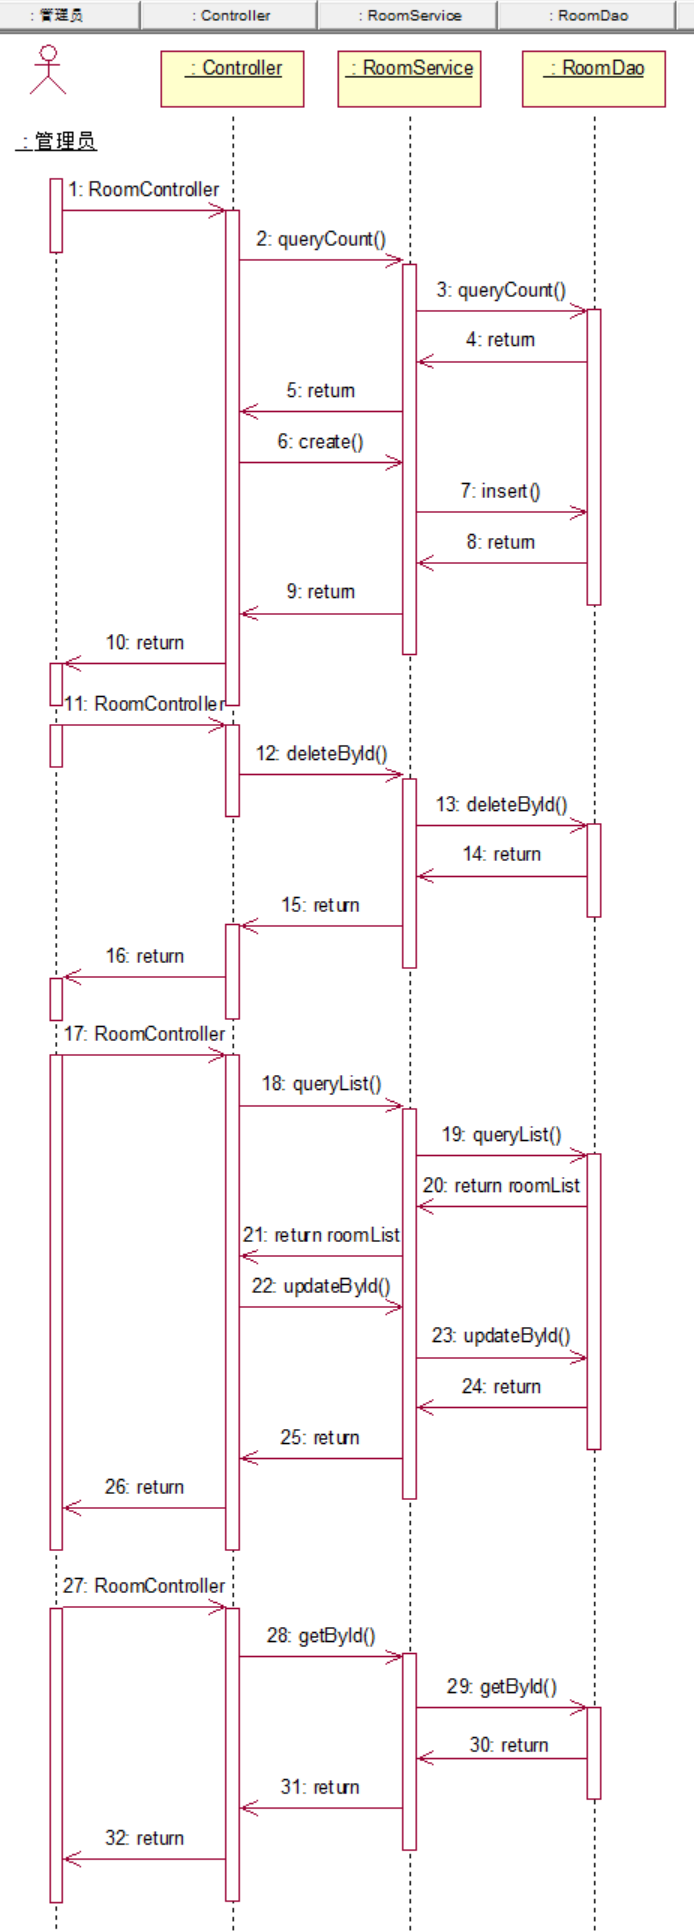
\includegraphics[width=0.9\textwidth,height=0.7\textheight,keepaspectratio]{figures/fig4-10.png}
  \caption{会议室管理模块顺序图}
  \label{fig:4-10}
\end{figure}

\subsection{报修管理模块顺序图设计}
用户进入报修管理界面，系统调用 RepariController 类中的查询接口，界面显示报修信息。用户在进行其他操作时，调用此类中的相应接口，Service 层进行业务逻辑处理，再通过调用 Dao 层与数据库交互，根据原路径，将信息显示到界面。报修管理模块顺序图如图~\ref{fig:4-11}~所示。

\begin{figure}[htbp]
  \centering
  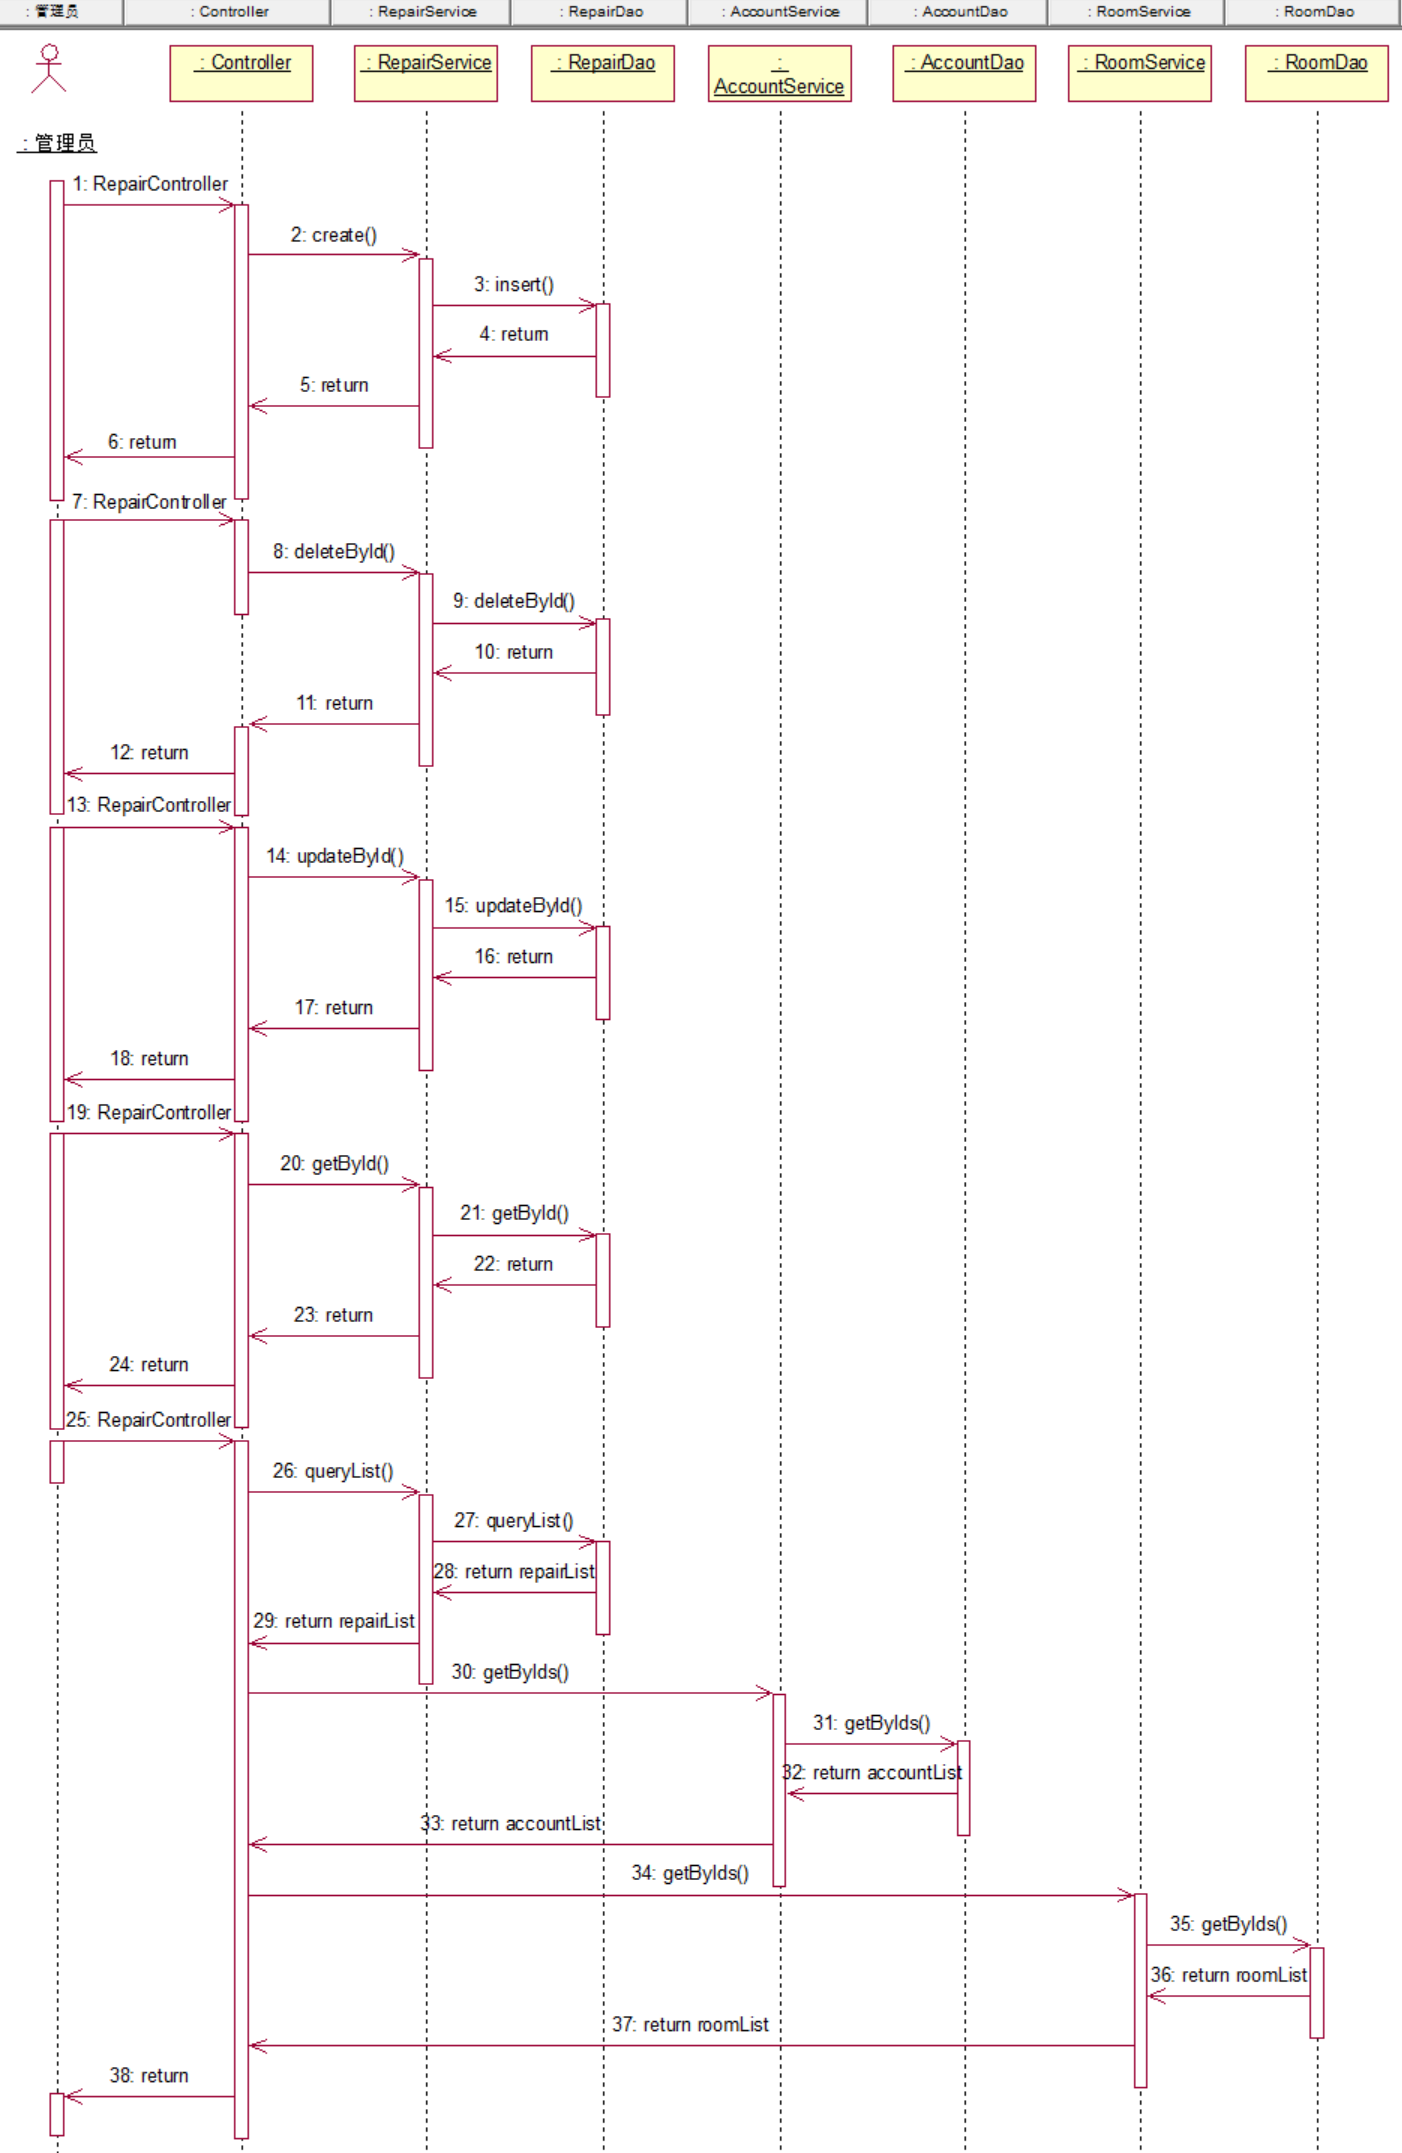
\includegraphics[width=0.9\textwidth,height=0.7\textheight,keepaspectratio]{figures/fig4-11.png}
  \caption{报修管理模块顺序图}
  \label{fig:4-11}
\end{figure}

\subsection{预约记录管理模块顺序图设计}
用户进入预约记录管理界面，系统调用 ReserveController 类中的查询接口，界面显示预约记录信息。根据用户选择的查询条件，调用此类中的相应接口，Service 层进行业务逻辑处理，再通过调用 Dao 层与数据库交互，根据原路径，将信息显示到界面。预约记录管理模块顺序图如图~\ref{fig:4-12}~所示。

\begin{figure}[htbp]
  \centering
  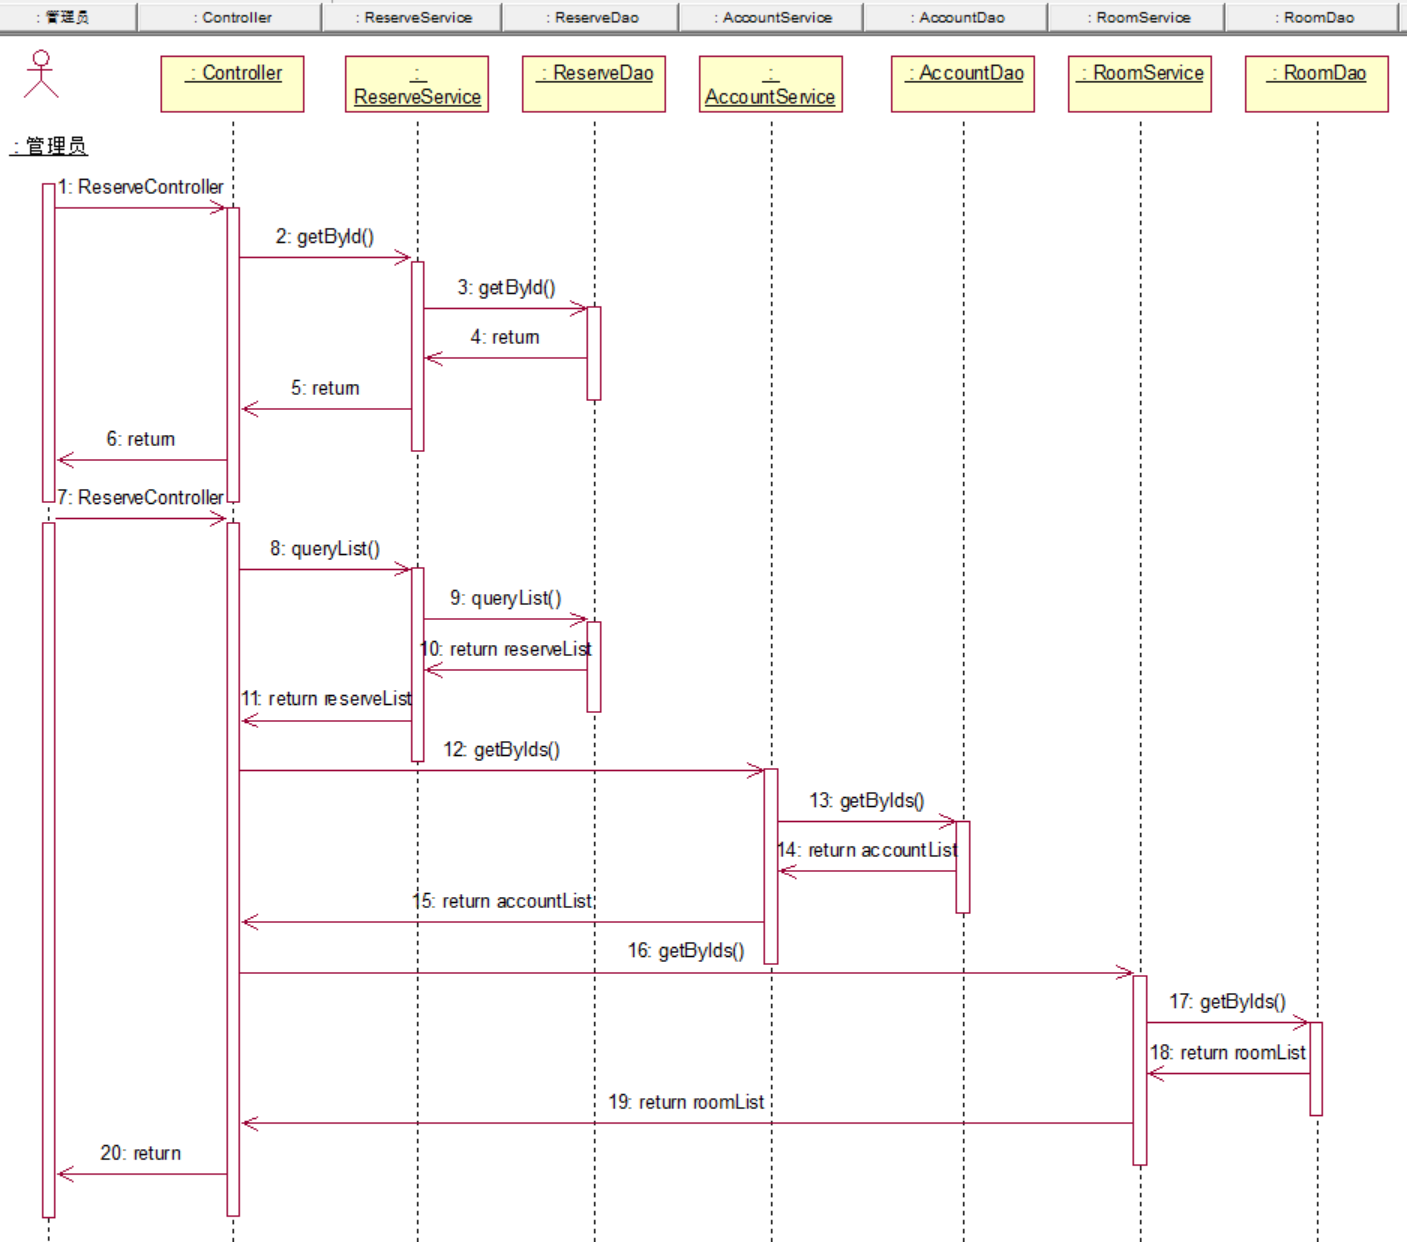
\includegraphics[width=0.9\textwidth,height=0.7\textheight,keepaspectratio]{figures/fig4-12.png}
  \caption{预约记录管理模块顺序图}
  \label{fig:4-12}
\end{figure}

\subsection{角色管理模块顺序图设计}
用户进入角色管理界面，系统调用 RoleController 类中的查询接口，界面显示角色信息。用户在进行其他操作时，调用此类中的相应接口，Service 层进行业务逻辑处理，再通过调用 Dao 层与数据库交互，根据原路径，将信息显示到界面。角色管理模块顺序图如图~\ref{fig:4-13}~所示。

\begin{figure}[htbp]
  \centering
  \includegraphics[width=0.9\textwidth,height=0.7\textheight,keepaspectratio]{figures/fig4-13.png}
  \caption{角色管理模块顺序图}
  \label{fig:4-13}
\end{figure}

\subsection{用户管理模块顺序图设计}
用户进入用户管理界面，系统调用 AccountController 类中的查询接口，界面显示用户信息。用户在进行其他操作时，调用此类中的相应接口，Service 层进行业务逻辑处理，再通过调用 Dao 层与数据库交互，根据原路径，将信息显示到界面。用户管理模块顺序图如图~\ref{fig:4-14}~所示。

\begin{figure}[htbp]
  \centering
  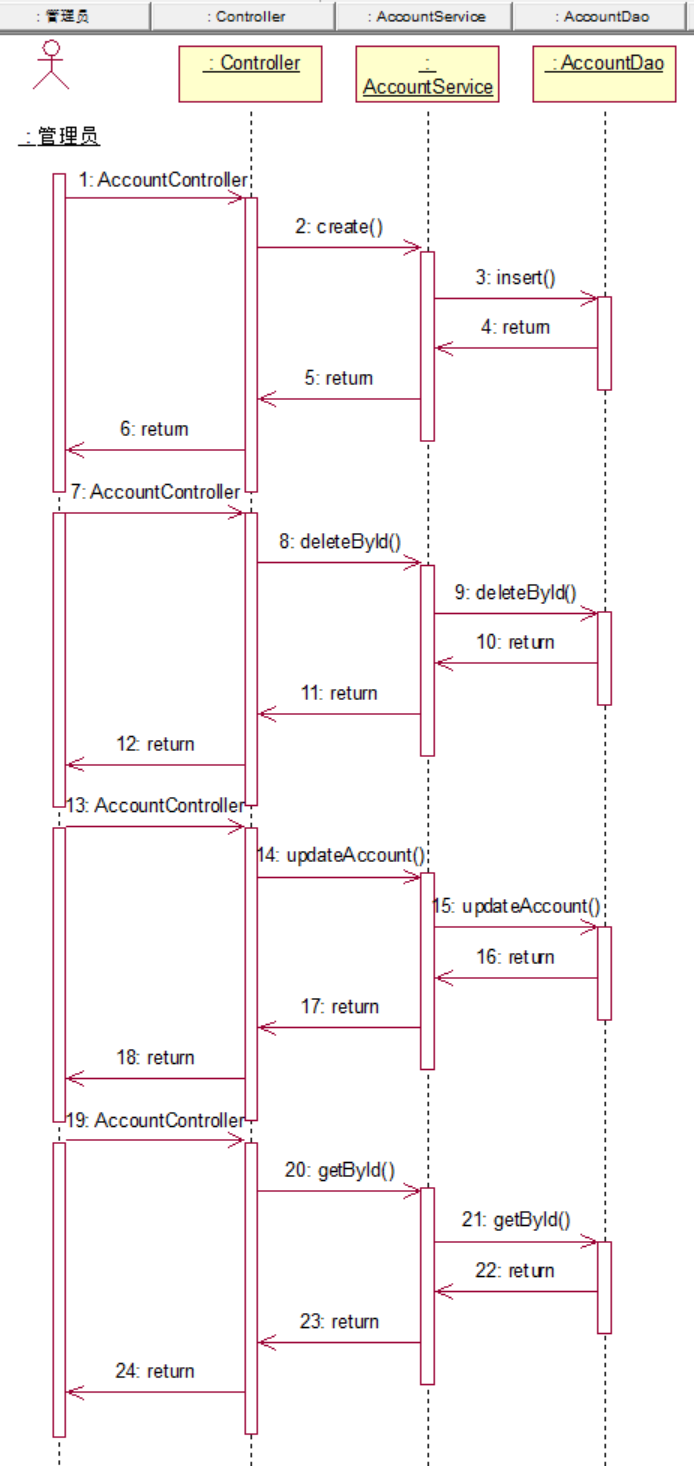
\includegraphics[width=0.9\textwidth,height=0.7\textheight,keepaspectratio]{figures/fig4-14.png}
  \caption{用户管理模块顺序图}
  \label{fig:4-14}
\end{figure}

\section{组件图}
组件图可以清晰地反映出会议室预约管理系统的结构，有利于理解系统，便于开发。下面如图~\ref{fig:4-15}~为系统组件图，如图~\ref{fig:4-16}~为系统主要业务组件图。

（1）会议室预约管理系统组件图

\begin{figure}[htbp]
  \centering
  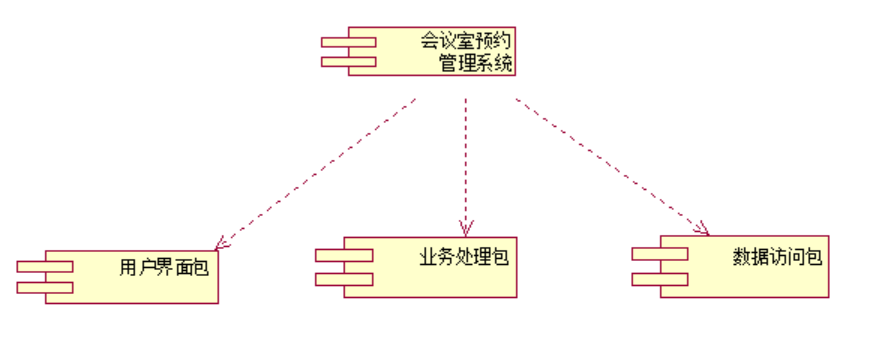
\includegraphics[width=0.8\textwidth]{figures/fig4-15.png}
  \caption{系统组件图}
  \label{fig:4-15}
\end{figure}

（2）系统主要业务组件图

\begin{figure}[htbp]
  \centering
  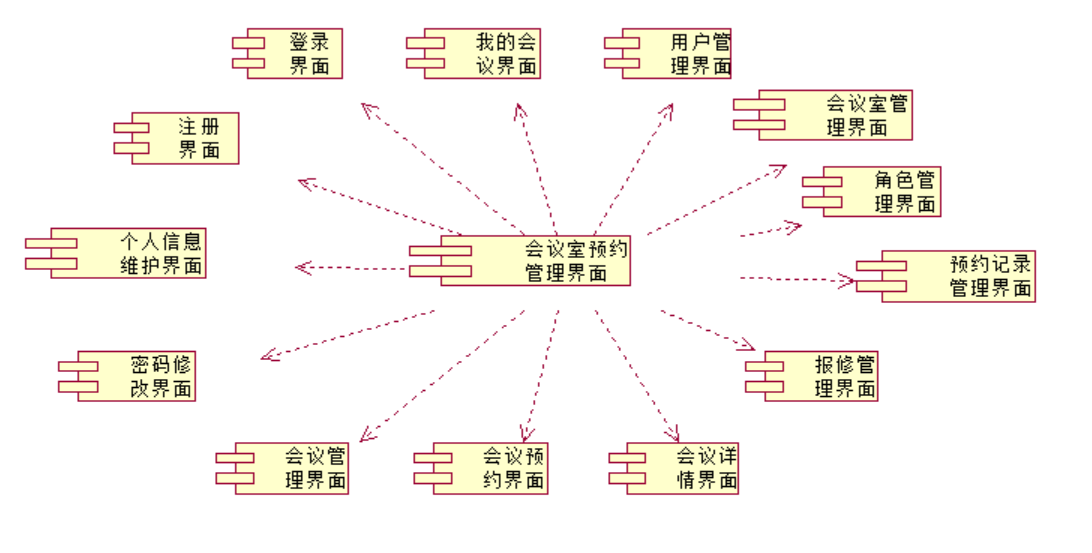
\includegraphics[width=0.9\textwidth]{figures/fig4-16.png}
  \caption{系统主要业务组件图}
  \label{fig:4-16}
\end{figure}

\section{部署图}
绘制部署图可以更好地描述系统运行时的结构及其部署情况，同时，也可以很直观地理解分布式系统。本系统的部署图如图~\ref{fig:4-17}~所示：

\begin{figure}[htbp]
  \centering
  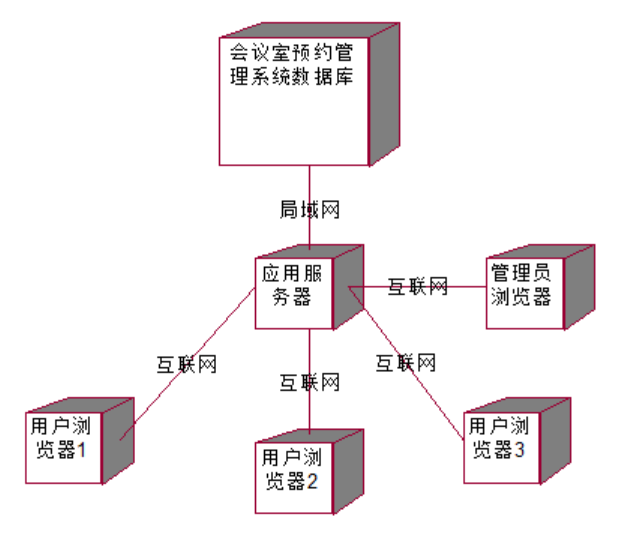
\includegraphics[width=0.55\textwidth]{figures/fig4-17.png}
  \caption{会议室预约管理系统部署图}
  \label{fig:4-17}
\end{figure}

\section{数据库设计}
\subsection{系统需求分析}
经过研究分析，本系统涉及以下七个实体：
\begin{itemize}
  \item 用户：属性有用户 ID、用户账号、用户名称、密码、用户状态、邮箱、角色、地址、手机号、性别、最近登录时间；
  \item 会议室：属性有会议室 ID、会议室名称、备注、实景照片、修改时间、创建时间；
  \item 会议：属性有会议 ID、会议名称、会议内容、人员名称、创建时间、修改时间；
  \item 报修：属性有报修 ID、报修状态、会议内容、修改时间、创建时间、报修人；
  \item 图片：属性有图片 ID、图片名称、创建时间、修改时间；
  \item 角色：属性有角色 ID、角色名称、角色类型、权限列表、创建时间、修改时间、备注；
  \item 预约：属性有预约 ID、预约内容、预约人、开始时间、结束时间、创建时间、修改时间。
\end{itemize}

这些实体之间的联系如下：

一个用户可以预约多个会议，一个会议只能由一个用户预约；一个用户可以查询多个会议室，一个会议室只能由一个用户查询；一个会议室包含一张图片，一张图片只能由一个会议室包含；一个用户可以查看多个会议详情，一个会议详情只能由一个用户查看；一个用户可以管理多个角色，一个角色只能由一个用户管理；一个用户可以管理多个报修记录，一个报修记录只能由一个用户管理。

\subsection{概念结构设计}
需求分析结束之后需进行概念结构设计，在数据库设计中其处于关键的地位。而 E-R 图是用来描述现实世界概念结构模型的方法，可以表示实体、属性以及实体之间的联系\cite{ref9}。根据需求分析得到的实体类、属性以及实体之间的联系设计本系统的 E-R 图如图~\ref{fig:4-18}~所示：

\begin{figure}[htbp]
  \centering
  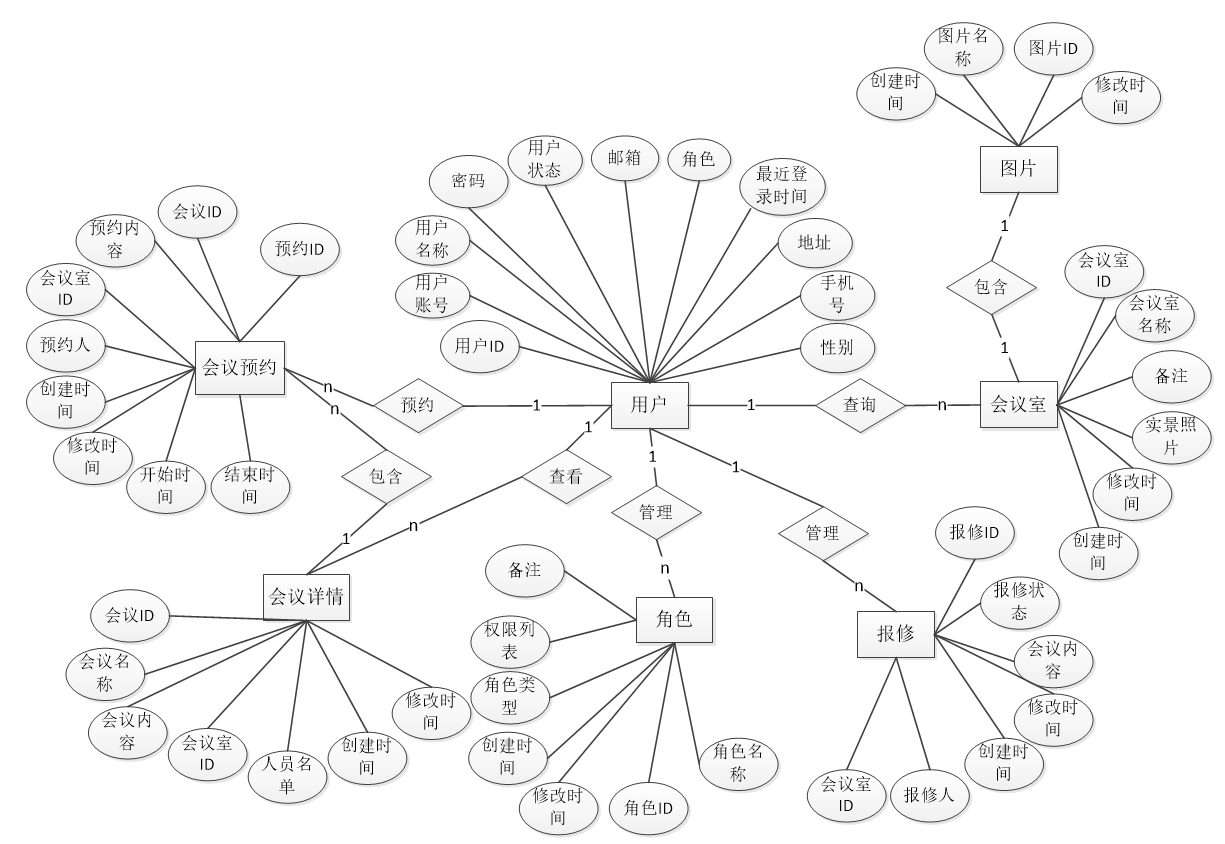
\includegraphics[width=\textwidth]{figures/fig4-18.png}
  \caption{会议室预约管理系统 E-R 图}
  \label{fig:4-18}
\end{figure}

\subsection{逻辑结构设计}
在得到系统 E-R 图后，需要将其转换为关系模型。在转换时的规则有：当是 1：1 的联系时，可以将任意一个实体的主键加入另一关系模式的属性中；当是 1：n 的联系时，在 n 端中加入 1 端的主键；当是 n：n 的联系时，主键为两端实体主键的组合\cite{ref10}。按照此转换规则得到的关系模式如下：

用户（用户 ID、用户账号、用户名称、密码、用户状态、邮箱、角色、地址、手机号、性别、最近登录时间），其中主键为用户 ID；

会议室（会议室 ID、会议室名称、备注、实景照片、修改时间、创建时间），其中主键为会议室 ID 与实景照片；

会议（会议 ID、会议名称、会议内容、人员名单、创建时间、修改时间、会议室 ID），其中主键为会议 ID，外键为会议室 ID 与人员名单；

报修（报修 ID、报修状态、会议内容、修改时间、创建时间、报修人、会议室 ID），其中主键为报修 ID，外键为会议室 ID 与报修人；

图片（图片 ID、图片名称、创建时间、修改时间），其中主键为图片 ID；

角色（角色 ID、角色名称、角色类型、权限列表、创建时间、修改时间、备注），其中主键为角色 ID；

预约（预约 ID、预约内容、预约人、开始时间、结束时间、创建时间、修改时间、会议 ID、会议室 ID），其中主键为预约 ID，外键为会议 ID、会议室 ID 与预约人。

\subsection{物理结构设计}
逻辑结构设计完成之后，确定数据库的物理结构，其包括数据的存放位置与存储结构。本系统的数据库设计如以下表所示：

用户账户表 account 如表~\ref{tab:4-1}~所示。

\begin{table}[htbp]
  \centering
  \caption{用户账户表 account}
  \label{tab:4-1}
  \zihao{5}\songti
  \begin{tabular}{|c|c|c|c|c|}
    \hline
    字段名 & 字段描述 & 数据类型 & 主键 & 外键 \\
    \hline
    id & 用户 ID & bigint & True & False \\
    \hline
    passport & 用户账号 & varchar & False & False \\
    \hline
    name & 用户名称 & varchar & False & False \\
    \hline
    password & 密码 & varchar & False & False \\
    \hline
    status & 用户状态 & int & False & False \\
    \hline
    role\_id & 角色 & bigint & False & False \\
    \hline
    email & 邮箱 & varchar & False & False \\
    \hline
    phone & 手机号 & varchar & False & False \\
    \hline
    address & 地址 & varchar & False & False \\
    \hline
    sex & 性别 & int & False & False \\
    \hline
    last\_login\_time & 最近登录时间 & bigint & False & False \\
    \hline
  \end{tabular}
\end{table}

会议表 meeting 如表~\ref{tab:4-2}~所示。

\begin{table}[htbp]
  \centering
  \caption{会议表 meeting}
  \label{tab:4-2}
  \zihao{5}\songti
  \begin{tabular}{|c|c|c|c|c|}
    \hline
    字段名 & 字段描述 & 数据类型 & 主键 & 外键 \\
    \hline
    id & 会议 ID & bigint & True & False \\
    \hline
    name & 会议名称 & varchar & False & False \\
    \hline
    content & 会议内容 & varchar & False & False \\
    \hline
    room\_id & 会议室 ID & bigint & False & True \\
    \hline
    account\_ids & 人员名单 & varchar & False & True \\
    \hline
    create\_time & 创建时间 & bigint & False & False \\
    \hline
    update\_time & 修改时间 & bigint & False & False \\
    \hline
  \end{tabular}
\end{table}

报修表 repair 如表~\ref{tab:4-3}~所示。

\begin{table}[htbp]
  \centering
  \caption{报修表 repair}
  \label{tab:4-3}
  \zihao{5}\songti
  \begin{tabular}{|c|c|c|c|c|}
    \hline
    字段名 & 字段描述 & 数据类型 & 主键 & 外键 \\
    \hline
    id & 报修 ID & bigint & True & False \\
    \hline
    statu & 报修状态 & int & False & False \\
    \hline
    content & 会议内容 & text & False & False \\
    \hline
    room\_id & 会议室 ID & bigint & False & True \\
    \hline
    account\_id & 报修人 & bigint & False & True \\
    \hline
    create\_time & 创建时间 & bigint & False & False \\
    \hline
    update\_time & 修改时间 & bigint & False & False \\
    \hline
  \end{tabular}
\end{table}

图片表 image 如表~\ref{tab:4-4}~所示。

\begin{table}[htbp]
  \centering
  \caption{图片表 image}
  \label{tab:4-4}
  \zihao{5}\songti
  \begin{tabular}{|c|c|c|c|c|}
    \hline
    字段名 & 字段描述 & 数据类型 & 主键 & 外键 \\
    \hline
    id & 图片 ID & bigint & True & False \\
    \hline
    name & 图片名称 & varchar & False & False \\
    \hline
    create\_time & 创建时间 & bigint & False & False \\
    \hline
    update\_time & 修改时间 & bigint & False & False \\
    \hline
  \end{tabular}
\end{table}

预约表 reserve 如表~\ref{tab:4-5}~所示。

\begin{table}[htbp]
  \centering
  \caption{预约表 reserve}
  \label{tab:4-5}
  \zihao{5}\songti
  \begin{tabular}{|c|c|c|c|c|}
    \hline
    字段名 & 字段描述 & 数据类型 & 主键 & 外键 \\
    \hline
    id & 预约 ID & bigint & True & False \\
    \hline
    meeting\_id & 会议 ID & bigint & False & True \\
    \hline
    content & 预约内容 & text & False & False \\
    \hline
    room\_id & 会议室 ID & bigint & False & True \\
    \hline
    account\_id & 预约人 & bigint & False & True \\
    \hline
    create\_time & 创建时间 & bigint & False & False \\
    \hline
    update\_time & 修改时间 & bigint & False & False \\
    \hline
    reserve\_start\_time & 开始时间 & bigint & False & False \\
    \hline
    reserve\_end\_time & 结束时间 & bigint & False & False \\
    \hline
  \end{tabular}
\end{table}

角色表 role 如表~\ref{tab:4-6}~所示。

\begin{table}[htbp]
  \centering
  \caption{角色表 role}
  \label{tab:4-6}
  \zihao{5}\songti
  \begin{tabular}{|c|c|c|c|c|}
    \hline
    字段名 & 字段描述 & 数据类型 & 主键 & 外键 \\
    \hline
    id & 角色 ID & bigint & True & False \\
    \hline
    name & 角色名称 & varchar & False & False \\
    \hline
    description & 备注 & varchar & False & False \\
    \hline
    authorities & 权限列表 & varchar & False & False \\
    \hline
    create\_time & 创建时间 & bigint & False & False \\
    \hline
    update\_time & 修改时间 & bigint & False & False \\
    \hline
    type & 角色类型 & int & False & False \\
    \hline
  \end{tabular}
\end{table}

会议室表 room 如表~\ref{tab:4-7}~所示。

\begin{table}[htbp]
  \centering
  \caption{会议室表 room}
  \label{tab:4-7}
  \zihao{5}\songti
  \begin{tabular}{|c|c|c|c|c|}
    \hline
    字段名 & 字段描述 & 数据类型 & 主键 & 外键 \\
    \hline
    id & 会议室 ID & bigint & True & False \\
    \hline
    name & 会议室名称 & varchar & False & False \\
    \hline
    description & 备注 & text & False & False \\
    \hline
    room\_image\_ids & 实景照片 & varchar & False & True \\
    \hline
    create\_time & 创建时间 & bigint & False & False \\
    \hline
    update\_time & 修改时间 & bigint & False & False \\
    \hline
  \end{tabular}
\end{table}

由于 MySQL 采用的是关系模型，其在数据存储方面更加方便用户查询数据，并且存储数据时根据数据表的结构，可以具有较高的可靠性和稳定性\cite{ref11}。在进行数据库中数据的增加、删除、修改、查询操作时，其结构化查询语言可以使操作更加方便。

正是由于其以上优点，本会议室预约管理系统采用 MySQL 来创建数据库，并进行数据管理。

\subsection{数据库实施}
完成数据库的物理设计之后，需要根据数据库逻辑设计与物理设计的结果编写 SQL 语句。本系统的建表 SQL 语句如下所示：

创建用户表：

\begin{center}
  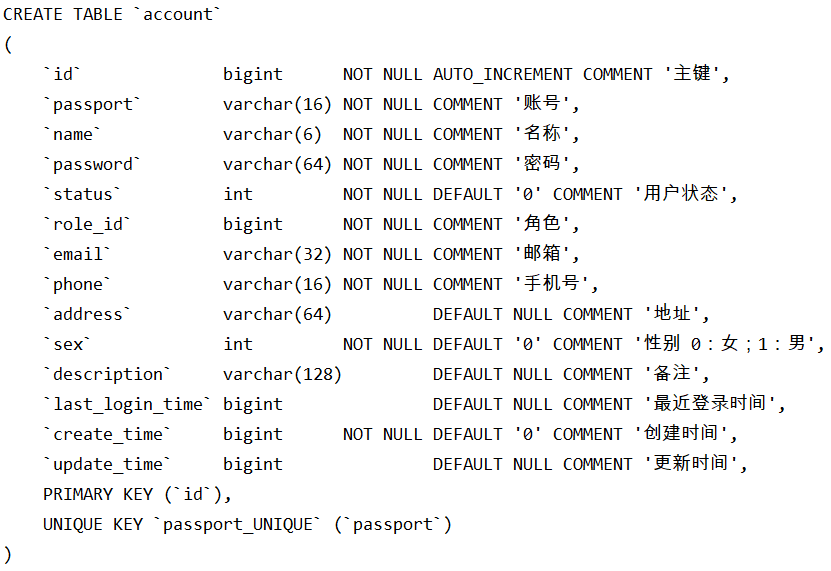
\includegraphics[width=0.8\textwidth]{figures/sql-account.png}
\end{center}

创建会议表：

\begin{center}
  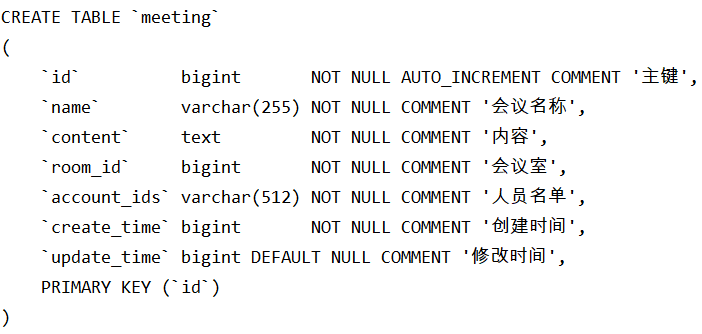
\includegraphics[width=0.8\textwidth]{figures/sql-meeting.png}
\end{center}

创建报修表：

\begin{center}
  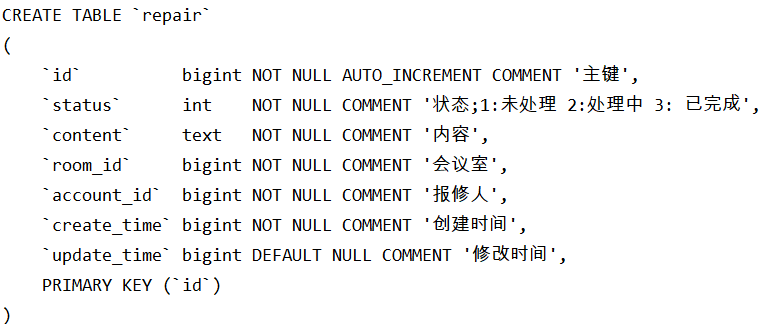
\includegraphics[width=0.8\textwidth]{figures/sql-repair.png}
\end{center}

创建预约表：

\begin{center}
  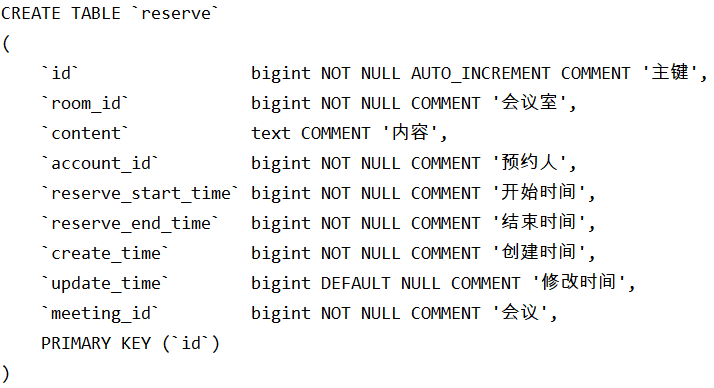
\includegraphics[width=0.8\textwidth]{figures/sql-reserve.png}
\end{center}

创建图片表：

\begin{center}
  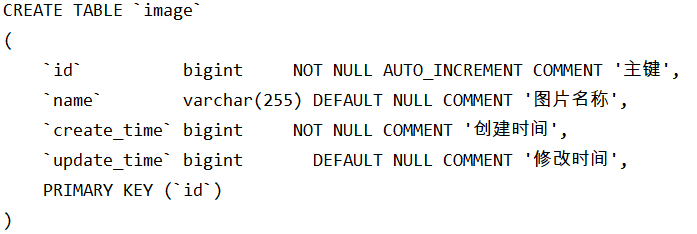
\includegraphics[width=0.8\textwidth]{figures/sql-image.png}
\end{center}

创建角色表：

\begin{center}
  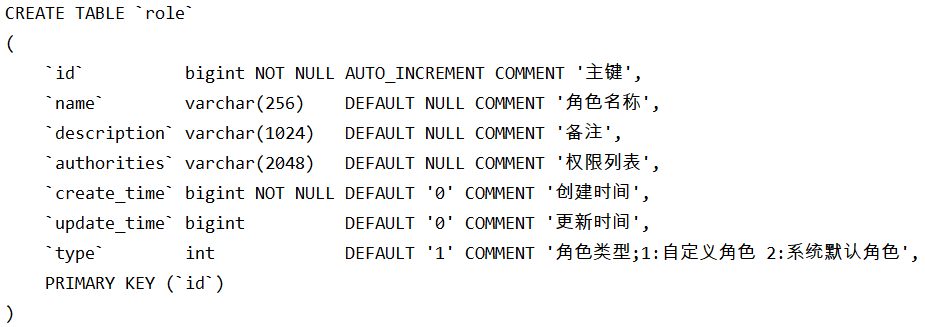
\includegraphics[width=0.8\textwidth]{figures/sql-role.png}
\end{center}

创建会议室表：

\begin{center}
  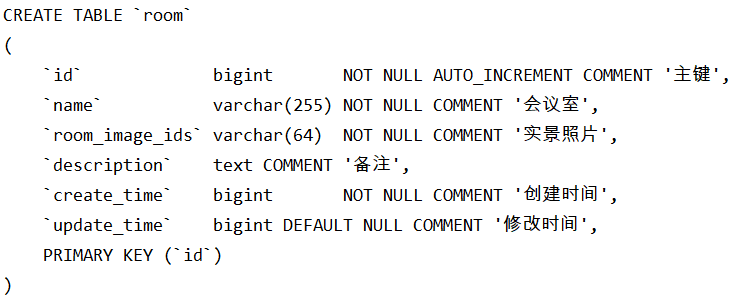
\includegraphics[width=0.8\textwidth]{figures/sql-room.png}
\end{center}

在创建完各个表结构之后，即可以在数据库中添加数据。先添加少量的数据试运行，待运行成功后再大批量输入数据。

\subsection{数据库运行与维护}
数据库维护是指当一个数据库被创建之后所做的所有工作。本系统主要通过进行备份来维护数据库。

数据备份是为了防止系统故障或人为操作失误等因素造成生产数据的丢失或损坏的\cite{ref12}。数据备份有三种方式，分别是全量备份、增量备份、差异备份。
\begin{itemize}
  \item 全量备份是指备份系统中的全部文件，但数据很多时会影响计算机性能。
  \item 增量备份是指仅仅将上一次备份后的操作进行备份，但其数据量很小。
  \item 差异备份是指将第一次备份后的操作进行备份，此方法数据量适中。
\end{itemize}

除了数据备份的方式之外，还可以进行数据库的备份。其备份有三种方式，分别是冷备份、热备份、逻辑备份\cite{ref13}。
\begin{itemize}
  \item 冷备份是指在不使用数据库时进行备份。其不太适用于数据库过大的情况。
  \item 热备份指的是当数据库中的数据有所更新时进行备份，但当系统在进行热备份的过程中崩溃时，会导致数据全部丢失。
  \item 逻辑备份是指通过使用软件从数据库中将数据提取到一个文件中，但不能对此文件做任何数据库的操作。
\end{itemize}

为了防止用户数据丢失，同时考虑到数据量适中，本系统选择定期进行差异备份以及冷备份。

\chapter{系统实现}

\section{会议室预约管理系统的多层架构}
会议室预约管理系统使用的是 Spring Boot 和 Vue 框架。实体层中实体类的属性值与数据库中的属性值是一致的；持久层即 Dao 层，其在与数据库交互中起作用，可以进行数据业务处理；业务层即 Service 层，可以进行业务逻辑处理；控制层即 Controller 层，其是用来控制业务流程的。

本部分以添加预约记录为例，阐述实现过程。

\subsection{实体类的设计与实现}
实体 Reserve 类对应预约表 reserve：

\begin{center}
  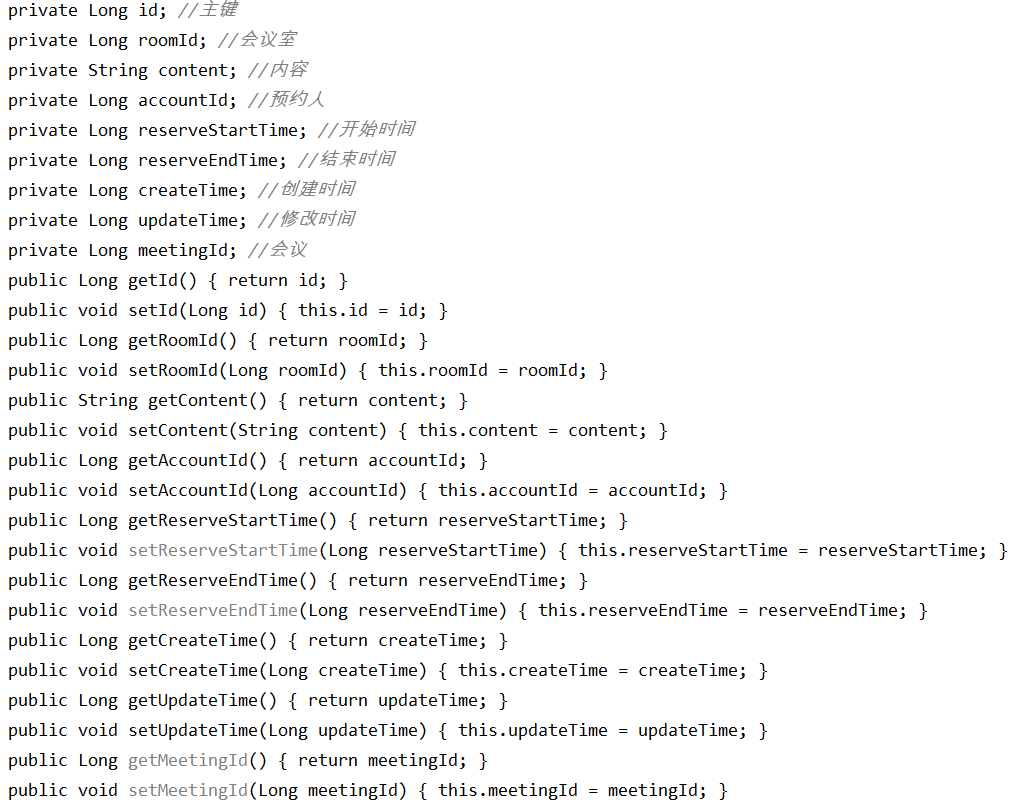
\includegraphics[width=0.85\textwidth]{figures/code-entity.png}
\end{center}

\subsection{持久层的设计与实现}
ReserveDao 中关于添加预约记录的部分代码:

\begin{center}
  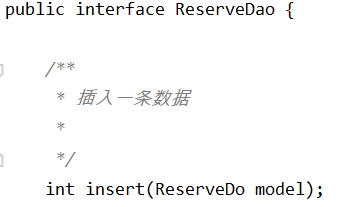
\includegraphics[width=0.85\textwidth]{figures/code-dao.png}
\end{center}

ReserveMapper.xml 中关于添加预约记录的部分代码:

\begin{center}
  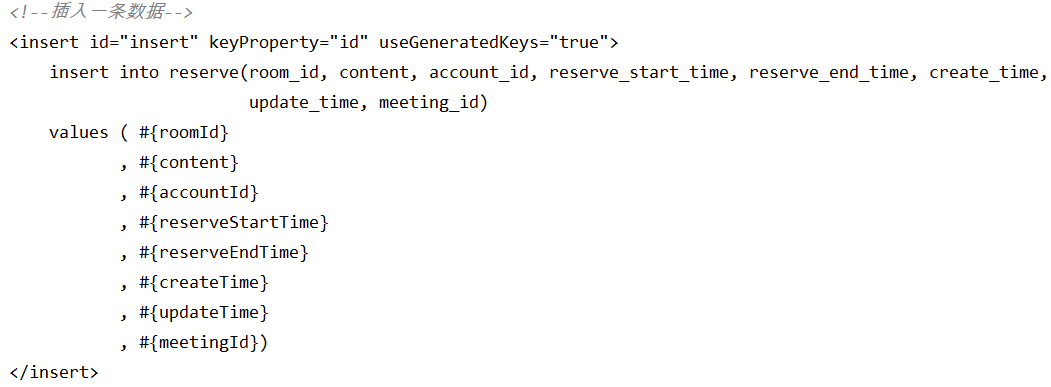
\includegraphics[width=0.85\textwidth]{figures/code-mapper.png}
\end{center}

\subsection{业务层的设计与实现}
ReserveServiceImpl 中关于添加预约记录的部分代码:

\begin{center}
  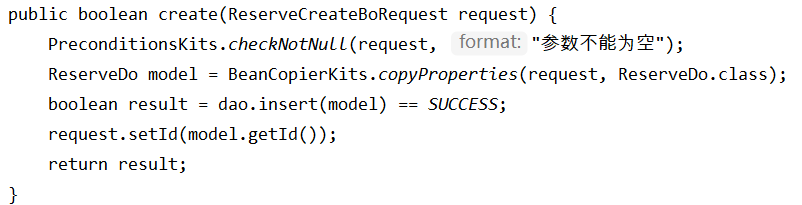
\includegraphics[width=0.85\textwidth]{figures/code-serviceimpl.png}
\end{center}

ReserveService 中关于添加预约记录的部分代码:

\begin{center}
  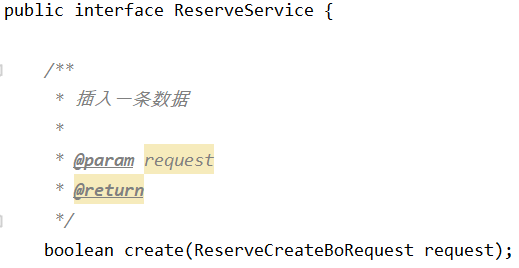
\includegraphics[width=0.85\textwidth]{figures/code-service.png}
\end{center}

\subsection{控制层的设计与实现}
ReserveController 中关于添加预约记录的部分代码:

\begin{center}
  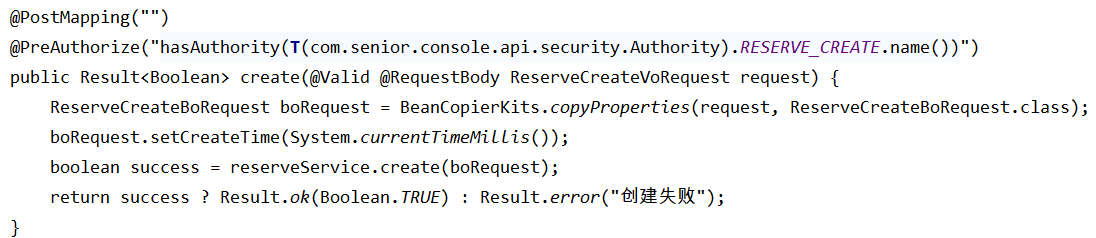
\includegraphics[width=0.85\textwidth]{figures/code-controller.png}
\end{center}

\section{会议室预约管理系统的实现}
会议室预约管理系统可以让用户在线预约会议并进行管理，提高资源利用率，节省用户时间。

1、用户登录界面

通过获取登录账号的 ID，获取此账号角色权限，区别普通用户与管理员，提供相应功能。用户登录界面如图~\ref{fig:5-1}~所示。

\begin{figure}[htbp]
  \centering
  \includegraphics[width=0.95\textwidth]{figures/fig5-1.png}
  \caption{用户登录界面}
  \label{fig:5-1}
\end{figure}

2、用户注册界面

用户在此界面进行注册，以便使用该系统功能。用户注册界面如图~\ref{fig:5-2}~所示。

\begin{figure}[htbp]
  \centering
  \includegraphics[width=0.95\textwidth]{figures/fig5-2.png}
  \caption{用户注册界面}
  \label{fig:5-2}
\end{figure}

3、我的会议界面

此界面以日历形式显示，用户在此界面可以清晰看到个人会议安排情况。我的会议界面如图~\ref{fig:5-3}~所示。

\begin{figure}[htbp]
  \centering
  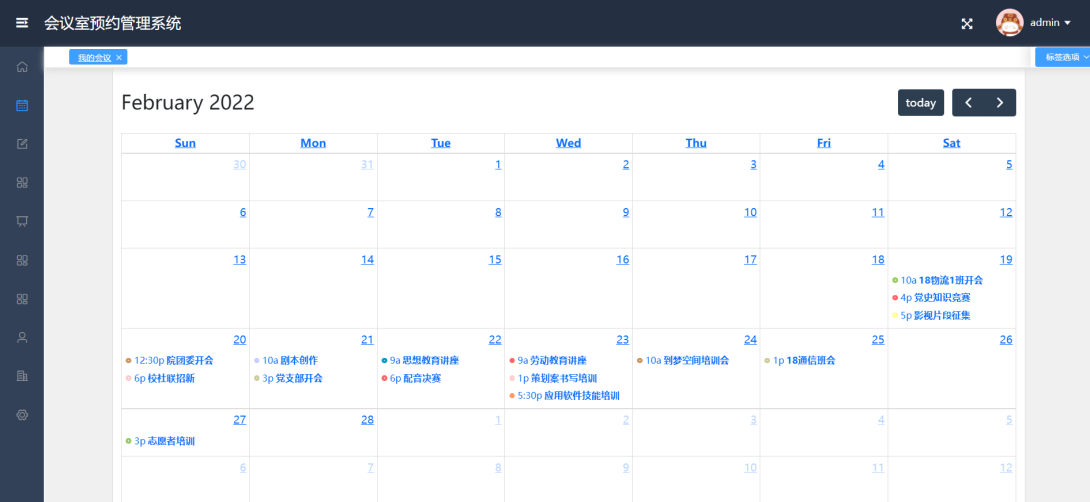
\includegraphics[width=0.95\textwidth]{figures/fig5-3.png}
  \caption{我的会议界面}
  \label{fig:5-3}
\end{figure}

4、个人信息维护界面

在此界面用户可以看到个人信息。并可根据需要修改个人相关信息。个人信息维护界面如图~\ref{fig:5-4}~所示。

\begin{figure}[htbp]
  \centering
  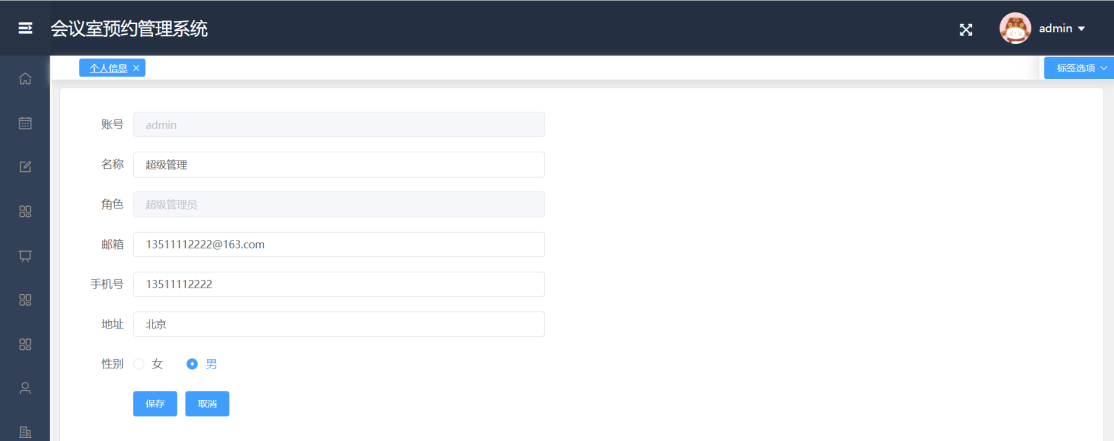
\includegraphics[width=0.95\textwidth]{figures/fig5-4.png}
  \caption{个人信息维护界面}
  \label{fig:5-4}
\end{figure}

5、密码修改界面

此界面输入相关信息可以修改个人密码。密码修改界面如图~\ref{fig:5-5}~所示。

\begin{figure}[htbp]
  \centering
  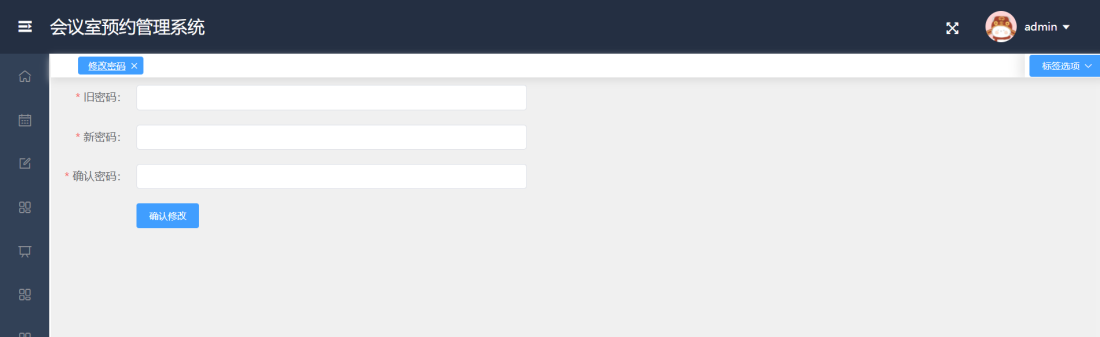
\includegraphics[width=0.95\textwidth]{figures/fig5-5.png}
  \caption{密码修改界面}
  \label{fig:5-5}
\end{figure}

6、会议预约界面

此界面显示了各个会议室的预约情况，通过在相应方块处拖拽，即可预约地点及时间，并进行保存。会议预约界面如图~\ref{fig:5-6}~所示。

\begin{figure}[htbp]
  \centering
  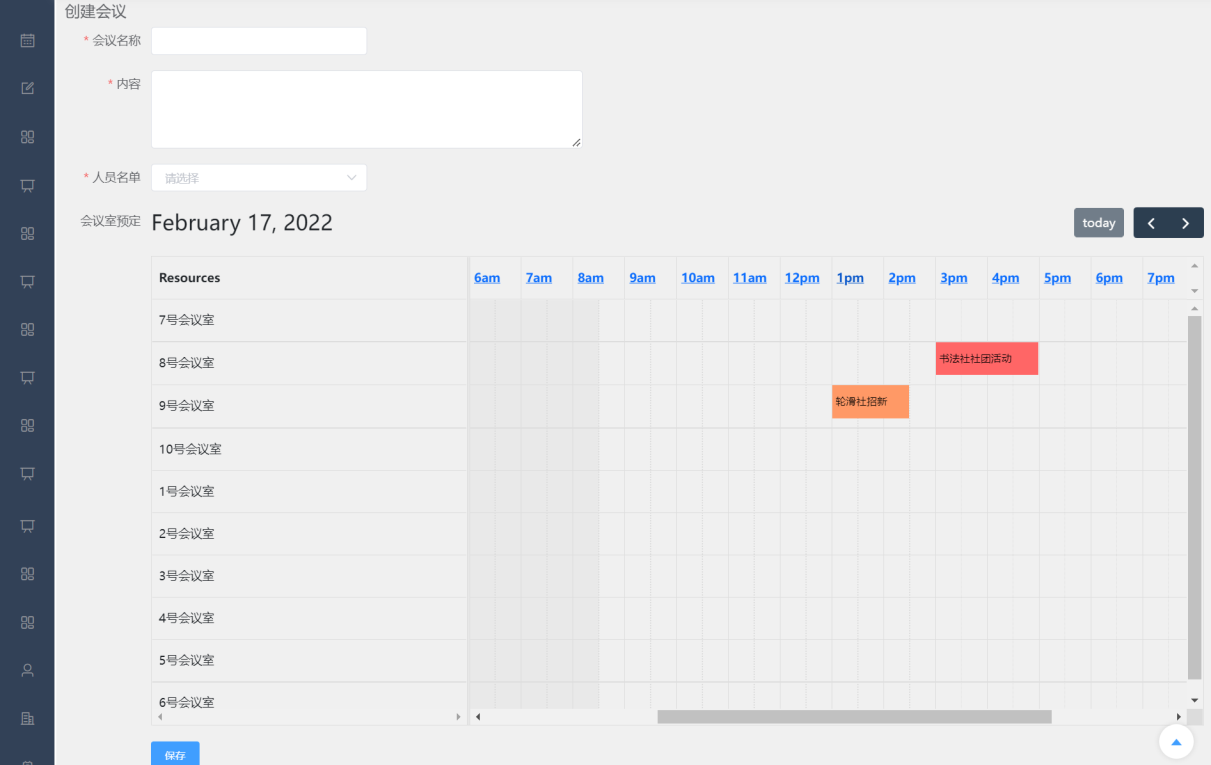
\includegraphics[width=0.95\textwidth]{figures/fig5-6.png}
  \caption{会议预约界面}
  \label{fig:5-6}
\end{figure}

7、会议管理界面

此界面显示了各个预约会议的大概信息，包括会议内容、参会人员、地点等信息，并可进行查询等其他操作。会议管理界面如图~\ref{fig:5-7}~所示。

\begin{figure}[htbp]
  \centering
  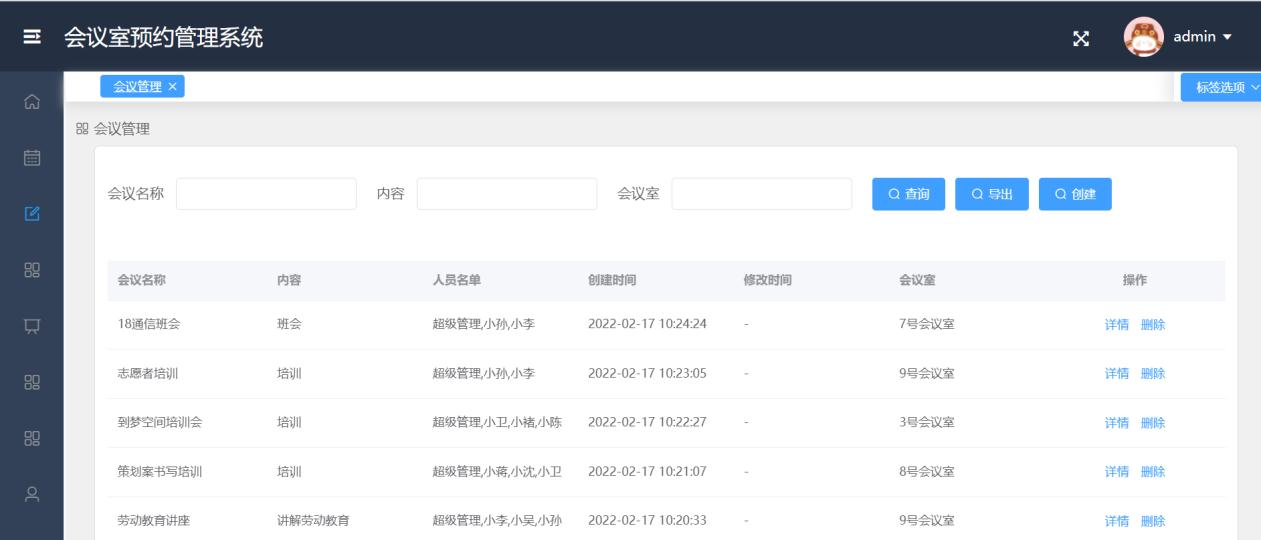
\includegraphics[width=0.95\textwidth]{figures/fig5-7.png}
  \caption{会议管理界面}
  \label{fig:5-7}
\end{figure}

8、会议详情界面

在此界面可以看到会议的详细信息，并可对其进行修改。会议详情界面如图~\ref{fig:5-8}~所示。

\begin{figure}[htbp]
  \centering
  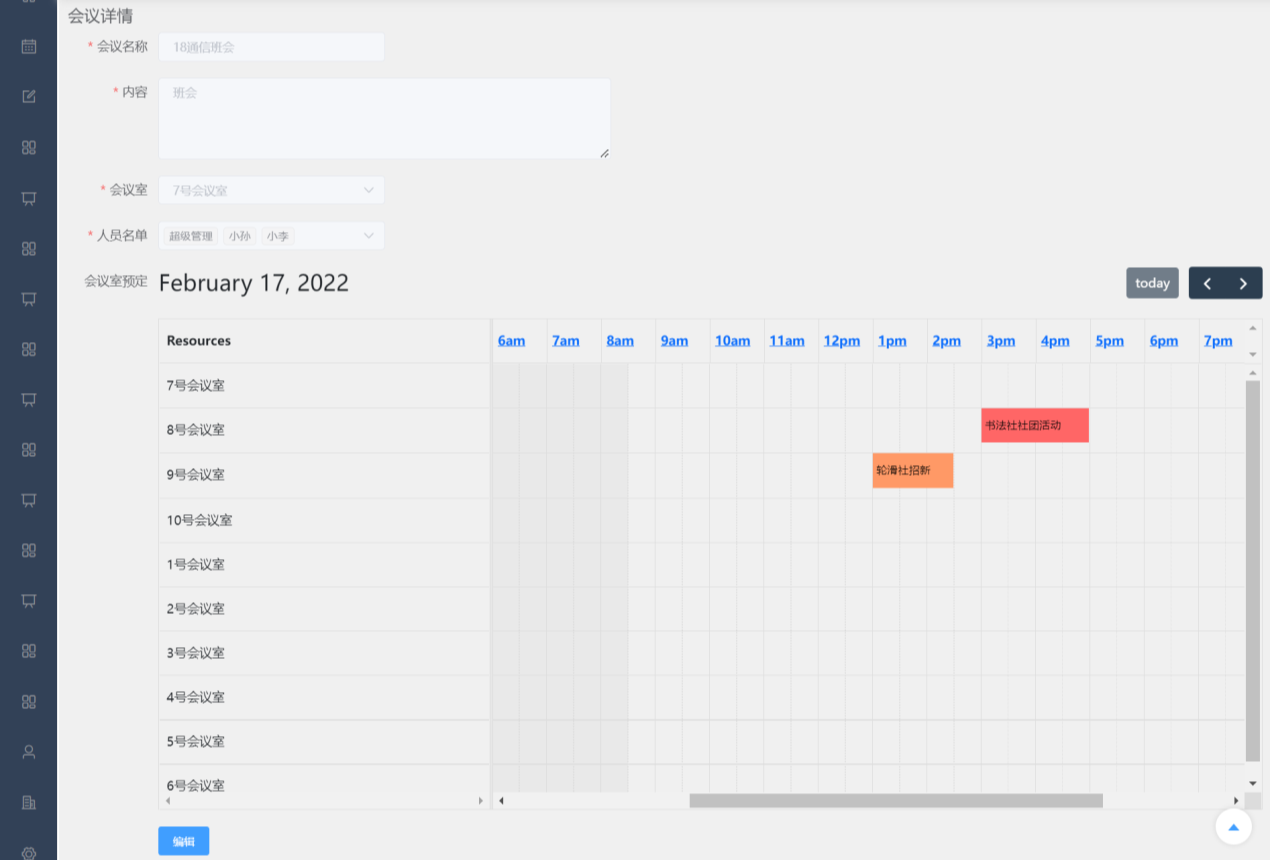
\includegraphics[width=0.95\textwidth]{figures/fig5-8.png}
  \caption{会议详情界面}
  \label{fig:5-8}
\end{figure}

9、报修管理界面

此界面可以看到各个报修记录情况，并可根据报修状态等进行搜索，以及其他操作。报修管理界面如图~\ref{fig:5-9}~所示。

\begin{figure}[htbp]
  \centering
  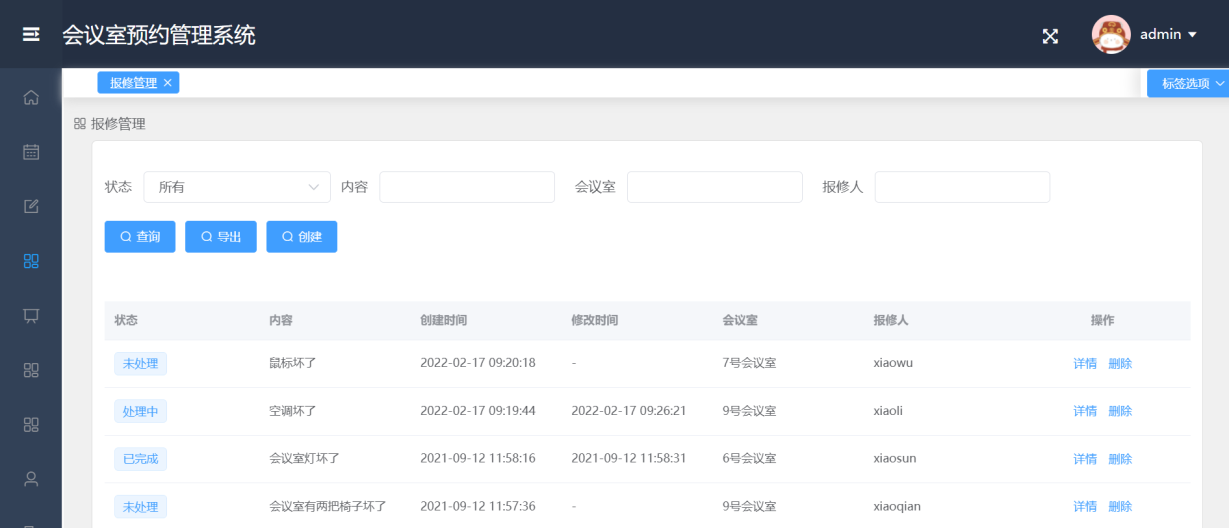
\includegraphics[width=0.95\textwidth]{figures/fig5-9.png}
  \caption{报修管理界面}
  \label{fig:5-9}
\end{figure}

10、报修详情界面

此界面可以修改报修情况，从而对会议室的维修状态进行标记。报修详情界面如图~\ref{fig:5-10}~所示。

\begin{figure}[htbp]
  \centering
  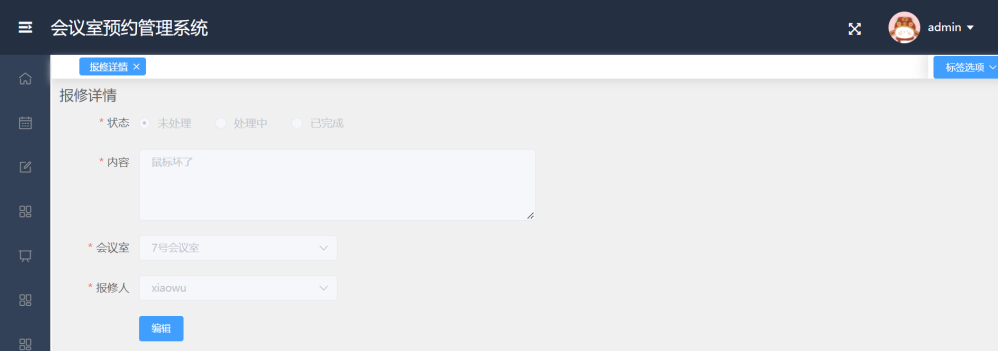
\includegraphics[width=0.95\textwidth]{figures/fig5-10.png}
  \caption{报修详情界面}
  \label{fig:5-10}
\end{figure}

11、预约记录管理界面

此界面主要根据条件进行预约记录查询，并可以显示各条预约记录情况。预约记录管理界面如图~\ref{fig:5-11}~所示。

\begin{figure}[htbp]
  \centering
  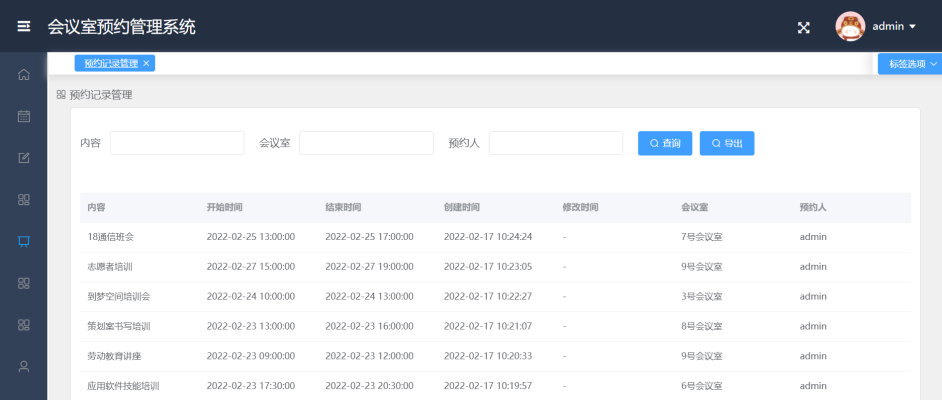
\includegraphics[width=0.95\textwidth]{figures/fig5-11.png}
  \caption{预约记录管理界面}
  \label{fig:5-11}
\end{figure}

12、会议室管理界面

通过此界面，用户可以查看各个会议室的配置情况，从而选择适合的会议室，且还可对其进行编辑。会议室管理界面如图~\ref{fig:5-12}~所示。

\begin{figure}[htbp]
  \centering
  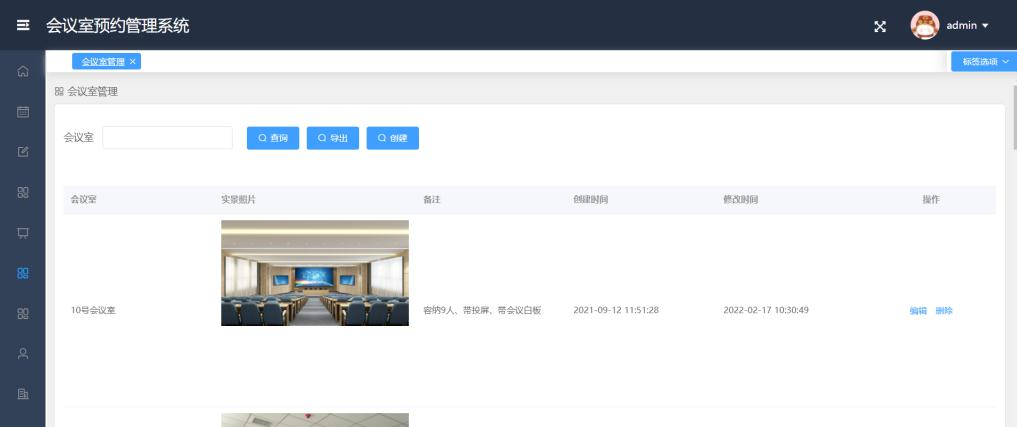
\includegraphics[width=0.95\textwidth]{figures/fig5-12.png}
  \caption{会议室管理界面}
  \label{fig:5-12}
\end{figure}

13、用户管理界面

管理员可以通过此界面，查询出符合条件的用户，并可对其进行编辑。用户管理界面如图~\ref{fig:5-13}~所示。

\begin{figure}[htbp]
  \centering
  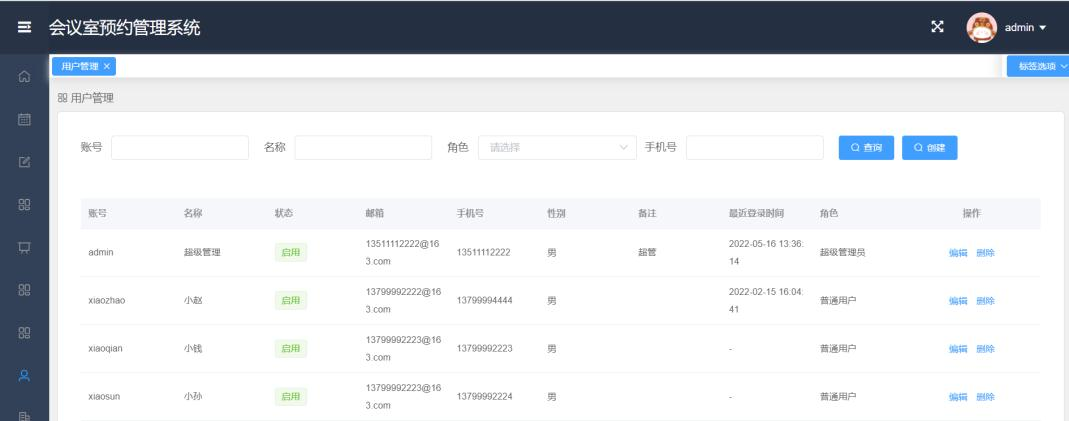
\includegraphics[width=0.95\textwidth]{figures/fig5-13.png}
  \caption{用户管理界面}
  \label{fig:5-13}
\end{figure}

14、角色管理界面

管理员可以通过此界面创建角色，且可对其权限进行设置。角色管理界面如图~\ref{fig:5-14}~所示。

\begin{figure}[htbp]
  \centering
  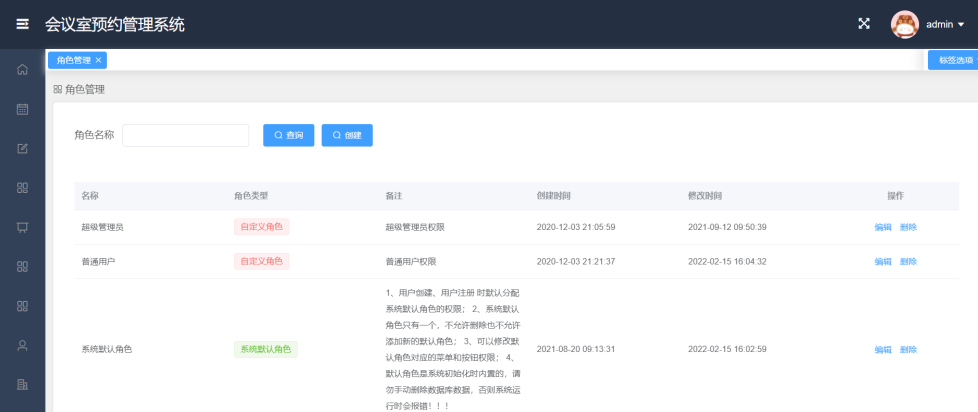
\includegraphics[width=0.95\textwidth]{figures/fig5-14.png}
  \caption{角色管理界面}
  \label{fig:5-14}
\end{figure}

\chapter{系统测试}

\section{测试目的}
系统测试处于非常重要的地位。通过系统测试，可以保证系统的质量，降低系统出现重大缺陷的几率，更好地符合用户的实际需求\cite{ref13}。所以为了完善系统，对会议室预约管理系统进行了系统测试。

\section{测试资源}
\subsection{硬件配置}
应用服务器：

处理器：Intel(R) Core(TM) i5-8250U CPU @ 1.60GHz

内存空间：12.0GB

硬盘空间：2TB

\subsection{软件配置}
数据库服务器操作系统：Navicat for MySQL

客户端操作系统：Windows 11

浏览器：Google

系统运行环境：JRE1.8

数据库管理系统：MySQL

其他：Microsoft Office 2016

\section{测试计划}
\subsection{测试方案}
采用黑盒测试方法验证会议室预约管理系统是否满足功能需求和非功能需求，编写测试用例时运用了等价类划分法和边界值法。

具体的测试用例如下：

1、登录模块测试；

2、注册模块测试；

3、个人信息维护模块测试；

4、密码修改模块测试；

5、会议预约模块测试；

6、会议管理模块测试；

7、报修管理模块测试；

8、预约记录管理模块测试；

9、会议室管理模块测试；

10、用户管理模块测试；

11、角色管理模块测试；

12、退出登录模块测试。

\subsection{典型测试用例}
以下测试用例的编写使用了等价类划分法和边界值法，他们都属于黑盒测试。其中等价类划分法是指将可能的输入数据划分为多个等价类，从每个等价类中选择代表性的数据作为测试用例。边界值法是对输入或输出的各种边界情况设计测试用例。

1、用户登录模块测试

{\zihao{5}\songti
\begin{longtable}{|p{2.3cm}|p{1.8cm}|p{1.9cm}|p{3.2cm}|p{2.1cm}|p{2.3cm}|}
  \hline
  测试编号 & 测试项目 & 预置条件 & 输入 & 执行步骤 & 预期输出 \\
  \hline
  \endfirsthead
  \hline
  测试编号 & 测试项目 & 预置条件 & 输入 & 执行步骤 & 预期输出 \\
  \hline
  \endhead
  HYSYY-TC01-001 & 登录模块测试 & 用户注册成功 & 正确的账号名：admin正确的密码：li123456 & 输入信息，点击登录 & 登录成功，跳转到系统首页 \\
  \hline
  HYSYY-TC01-002 & 登录模块测试 & 用户注册成功 & 错误的账号名：xiaoli正确的密码：li123456 & 输入信息，点击登录 & 登录失败，系统提示账号或密码错误 \\
  \hline
  HYSYY-TC01-003 & 登录模块测试 & 用户注册成功 & 正确的账号名：admin错误的密码：111111 & 输入信息，点击登录 & 登录失败，系统提示账号或密码错误 \\
  \hline
  HYSYY-TC01-004 & 登录模块测试 & 用户注册成功 & 无 & 点击登录 & 登录失败，系统提示请输入账号和密码 \\
  \hline
  HYSYY-TC01-005 & 登录模块测试 & 用户注册成功 & 正确的账号名：admin密码为空 & 点击登录 & 登录失败，系统提示密码错误 \\
  \hline
  HYSYY-TC01-006 & 登录模块测试 & 用户注册成功 & 不输入账号名正确的密码：li123456 & 点击登录 & 登录失败，系统提示账号名不能为空 \\
  \hline
\end{longtable}
}

2、个人信息维护模块测试

{\zihao{5}\songti
\begin{longtable}{|p{2.3cm}|p{1.8cm}|p{1.9cm}|p{3.2cm}|p{2.1cm}|p{2.3cm}|}
  \hline
  测试编号 & 测试项目 & 预置条件 & 输入 & 执行步骤 & 预期输出 \\
  \hline
  \endfirsthead
  \hline
  测试编号 & 测试项目 & 预置条件 & 输入 & 执行步骤 & 预期输出 \\
  \hline
  \endhead
  HYSYY-TC02-001 & 个人信息维护模块测试 & 用户登录成功，且点击个人信息按钮 & 正确的名称：小燕；其他不变 & 输入信息，点击保存 & 系统提示成功 \\
  \hline
  HYSYY-TC02-002 & 个人信息维护模块测试 & 用户登录成功，且点击个人信息按钮 & 正确的邮箱：1174309294@qq.com；其他不变 & 输入信息后，点击保存 & 系统提示成功 \\
  \hline
  HYSYY-TC02-003 & 个人信息维护模块测试 & 用户登录成功，且点击个人信息按钮 & 正确的手机号：18365727287；其他不变 & 输入信息后，点击保存 & 系统提示成功 \\
  \hline
  HYSYY-TC02-004 & 个人信息维护模块测试 & 用户登录成功，且点击个人信息按钮 & 正确的地址：山东；其他不变 & 输入信息后，点击保存 & 系统提示成功 \\
  \hline
  HYSYY-TC02-005 & 个人信息维护模块测试 & 用户登录成功，且点击个人信息按钮 & 更改性别；其他不变 & 输入信息后，点击保存 & 系统提示成功 \\
  \hline
  HYSYY-TC02-006 & 个人信息维护模块测试 & 用户登录成功，且点击个人信息按钮 & 无更改 & 点击保存 & 跳转至个人信息界面 \\
  \hline
  HYSYY-TC02-007 & 个人信息维护模块测试 & 用户登录成功，且点击个人信息按钮 & 无更改 & 点击取消 & 跳转至个人信息界面 \\
  \hline
  HYSYY-TC02-008 & 个人信息维护模块测试 & 用户登录成功，且点击个人信息按钮 & 名称为空，其他不变 & 点击保存 & 系统提示名称不能为空 \\
  \hline
  HYSYY-TC02-009 & 个人信息维护模块测试 & 用户登录成功，且点击个人信息按钮 & 手机号为空，其他不变 & 点击保存 & 系统提示手机号不能为空 \\
  \hline
  HYSYY-TC02-010 & 个人信息维护模块测试 & 用户登录成功，且点击个人信息按钮 & 邮箱为空，其他不变 & 点击保存按钮 & 系统提示邮箱不能为空 \\
  \hline
  HYSYY-TC02-011 & 个人信息维护模块测试 & 用户登录成功，且点击个人信息按钮 & 地址为空，其他不变 & 点击保存按钮 & 系统提示地址不能为空 \\
  \hline
  HYSYY-TC02-012 & 个人信息维护模块测试 & 用户登录成功，且点击个人信息按钮 & 手机号为 10 位，其他不变 & 点击保存按钮 & 系统提示手机号错误 \\
  \hline
  HYSYY-TC02-013 & 个人信息维护模块测试 & 用户登录成功，且点击个人信息按钮 & 手机号为 12 位，其他不变 & 点击保存按钮 & 系统提示手机号错误 \\
  \hline
  HYSYY-TC02-014 & 个人信息维护模块测试 & 用户登录成功，且点击个人信息按钮 & 手机号含有特殊符号，其他不变 & 点击保存按钮 & 系统提示手机号错误 \\
  \hline
  HYSYY-TC02-015 & 个人信息维护模块测试 & 用户登录成功，且点击个人信息按钮 & 手机号含有小数点，其他不变 & 点击保存按钮 & 系统提示手机号错误 \\
  \hline
\end{longtable}
}

3、会议预约模块测试

{\zihao{5}\songti
\begin{longtable}{|p{2.3cm}|p{1.8cm}|p{1.9cm}|p{3.2cm}|p{2.1cm}|p{2.3cm}|}
  \hline
  测试编号 & 测试项目 & 预置条件 & 输入 & 执行步骤 & 预期输出 \\
  \hline
  \endfirsthead
  \hline
  测试编号 & 测试项目 & 预置条件 & 输入 & 执行步骤 & 预期输出 \\
  \hline
  \endhead
  HYSYY-TC03-001 & 会议预约模块测试 & 用户登录成功 & 正确的会议名称：社团活动；内容：社团培训人员；人员名单：选择人员；选择预约时间 & 输入信息后，点击保存按钮 & 系统提示创建成功 \\
  \hline
  HYSYY-TC03-002 & 会议预约模块测试 & 用户登录成功 & 正确的会议名称：图书馆社团活动；内容：社团培训人员；人员名单：选择人员；选择两个预约时间段 & 输入信息后，点击保存按钮 & 系统提示一次只能预约一个时间段 \\
  \hline
  HYSYY-TC03-003 & 会议预约模块测试 & 用户登录成功 & 正确的会议名称：团总支社团活动；内容：社团培训人员；人员名单：选择人员；选择预约时间小于当前时间 & 输入信息后，点击保存按钮 & 系统提示预约时间不能小于当前时间 \\
  \hline
  HYSYY-TC03-004 & 会议预约模块测试 & 用户登录成功 & 不输入会议名称；内容：社团培训人员；人员名单：选择人员；选择预约时间 & 输入信息后，点击保存按钮 & 系统提示请输入会议名称 \\
  \hline
  HYSYY-TC03-005 & 会议预约模块测试 & 用户登录成功 & 正确的会议名称：团总支社团活动；不输入内容；人员名单：选择人员；选择预约时间 & 输入信息后，点击保存按钮 & 系统提示请输入内容 \\
  \hline
  HYSYY-TC03-006 & 会议预约模块测试 & 用户登录成功 & 正确的会议名称：社团活动；内容：社团培训人员；不选择人员名单；选择预约时间 & 输入信息后，点击保存按钮 & 系统提示请输入人员名单 \\
  \hline
  HYSYY-TC03-007 & 会议预约模块测试 & 用户登录成功 & 正确的会议名称：社团活动；内容：社团培训人员；人员名单：选择人员；不选择预约时间 & 输入信息后，点击保存按钮 & 系统提示请选择预约时间 \\
  \hline
  HYSYY-TC03-008 & 会议预约模块测试 & 用户登录成功 & 无 & 点击保存按钮 & 系统提示请输入相关信息 \\
  \hline
  HYSYY-TC03-009 & 会议预约模块测试 & 用户登录成功 & 无 & 点击取消按钮 & 跳转至会议管理界面 \\
  \hline
\end{longtable}
}

4、报修管理测试

{\zihao{5}\songti
\begin{longtable}{|p{2.3cm}|p{1.8cm}|p{1.9cm}|p{3.2cm}|p{2.1cm}|p{2.3cm}|}
  \hline
  测试编号 & 测试项目 & 预置条件 & 输入 & 执行步骤 & 预期输出 \\
  \hline
  \endfirsthead
  \hline
  测试编号 & 测试项目 & 预置条件 & 输入 & 执行步骤 & 预期输出 \\
  \hline
  \endhead
  HYSYY-TC04-001 & 报修管理测试 & 管理员登录成功 & 选择未处理状态 & 点击查询按钮 & 显示未处理报修记录 \\
  \hline
  HYSYY-TC04-002 & 报修管理模块测试 & 管理员登录成功 & 选择处理中状态 & 点击查询按钮 & 显示处理中报修记录 \\
  \hline
  HYSYY-TC04-003 & 报修管理测试 & 管理员登录成功 & 选择已完成状态 & 点击查询按钮 & 显示已完成报修记录 \\
  \hline
  HYSYY-TC04-004 & 报修管理测试 & 管理员登录成功 & 选择所有状态 & 点击查询按钮 & 显示所有报修记录 \\
  \hline
  HYSYY-TC04-005 & 报修管理测试 & 管理员登录成功 & 选择所有状态，输入会议内容 & 点击查询按钮 & 显示符合条件的报修记录 \\
  \hline
  HYSYY-TC04-006 & 报修管理测试 & 管理员登录成功 & 选择所有状态，输入会议室 & 点击查询按钮 & 显示符合条件的报修记录 \\
  \hline
  HYSYY-TC04-007 & 报修管理测试 & 管理员登录成功 & 选择所有状态，输入报修人 & 点击查询按钮 & 显示符合条件的报修记录 \\
  \hline
  HYSYY-TC04-008 & 报修管理测试 & 管理员登录成功 & 选择会议室；选择报修人；输入报修内容 & 点击创建按钮，输入相关信息，点击保存 & 系统提示创建成功 \\
  \hline
  HYSYY-TC04-009 & 报修管理测试 & 管理员登录成功 & 不选择会议室；选择报修人；输入报修内容 & 点击创建按钮，输入相关信息，点击保存 & 系统提示请选择会议室 \\
  \hline
  HYSYY-TC04-010 & 报修管理测试 & 管理员登录成功 & 选择会议室；不选择报修人；输入报修内容 & 点击创建按钮，输入相关信息，点击保存 & 系统提示请选择报修人 \\
  \hline
  HYSYY-TC04-011 & 报修管理测试 & 管理员登录成功 & 选择会议室；选择报修人；不输入报修内容 & 点击创建按钮，输入相关信息，点击保存 & 系统提示请输入内容 \\
  \hline
  HYSYY-TC04-012 & 报修管理测试 & 管理员登录成功 & 无 & 点击保存 & 系统提示请输入相关信息 \\
  \hline
  HYSYY-TC04-013 & 报修管理测试 & 管理员登录成功 & 无 & 点击删除按钮 & 成功删除 \\
  \hline
  HYSYY-TC04-014 & 报修管理测试 & 管理员登录成功 & 无 & 点击详情按钮 & 跳转至报修详情界面 \\
  \hline
  HYSYY-TC04-015 & 报修管理测试 & 管理员登录成功 & 修改状态；其他不变 & 点击保存按钮 & 系统提示编辑成功 \\
  \hline
  HYSYY-TC04-016 & 报修管理测试 & 管理员登录成功 & 修改内容；其他不变 & 点击保存按钮 & 系统提示编辑成功 \\
  \hline
  HYSYY-TC04-017 & 报修管理测试 & 管理员登录成功 & 修改会议室；其他不变 & 点击保存按钮 & 系统提示编辑成功 \\
  \hline
  HYSYY-TC04-018 & 报修管理测试 & 管理员登录成功 & 修改报修人；其他不变 & 点击保存按钮 & 系统提示编辑成功 \\
  \hline
  HYSYY-TC04-019 & 报修管理测试 & 管理员登录成功 & 无 & 点击取消按钮 & 跳转至报修管理界面 \\
  \hline
  HYSYY-TC04-020 & 报修管理测试 & 管理员登录成功 & 无 & 点击导出按钮 & 成功导出报修记录 \\
  \hline
\end{longtable}
}

5、预约记录管理测试

{\zihao{5}\songti
\begin{longtable}{|p{2.3cm}|p{1.8cm}|p{1.9cm}|p{3.2cm}|p{2.1cm}|p{2.3cm}|}
  \hline
  测试编号 & 测试项目 & 预置条件 & 输入 & 执行步骤 & 预期输出 \\
  \hline
  \endfirsthead
  \hline
  测试编号 & 测试项目 & 预置条件 & 输入 & 执行步骤 & 预期输出 \\
  \hline
  \endhead
  HYSYY-TC05-001 & 预约记录管理测试 & 管理员登录成功 & 输入会议内容 & 点击查询按钮 & 显示符合条件会议记录 \\
  \hline
  HYSYY-TC05-002 & 预约记录管理测试 & 管理员登录成功 & 输入会议室 & 点击查询按钮 & 显示符合条件会议记录 \\
  \hline
  HYSYY-TC05-003 & 预约记录管理测试 & 管理员登录成功 & 输入预约人 & 点击查询按钮 & 显示符合条件会议记录 \\
  \hline
  HYSYY-TC05-004 & 预约记录管理测试 & 管理员登录成功 & 输入会议内容和会议室 & 点击查询按钮 & 显示符合条件会议记录 \\
  \hline
  HYSYY-TC05-005 & 预约记录管理测试 & 管理员登录成功 & 输入会议内容、会议室和预约人 & 点击查询按钮 & 显示符合条件会议记录 \\
  \hline
  HYSYY-TC05-006 & 预约记录管理测试 & 管理员登录成功 & 无 & 点击预约记录管理按钮 & 显示所有预约记录信息 \\
  \hline
\end{longtable}
}

\chapter{总结和展望}

\section{总结}
通过对目前会议室预约情况的调查以及对国内外预约系统的研究，发现用户使用此会议室预约管理系统进行会议预约及管理，不仅在一定程度上节省了个人时间及精力，且节省了人力资源，提高工作效率。因此制定了实现此系统的方案。按照软件工程的思想，进行了调研、需求分析、系统设计、系统实现以及系统测试。

在会议室预约管理系统的需求分析阶段，通过绘制用例图、类图以及活动图，更好地表达了用户的功能需求，并基于此设计了类图以及数据库。本系统采用 Spring Boot 和 Vue 架构，设计了多层框架。在开发该系统时使用的是具有强大功能的 IntelliJ IDEA，使开发更便捷，同时后台数据库使用的是 MySQL 来进行数据的存储。会议室预约管理系统的角色分为普通用户与管理员，其划分是通过使用权限的设置，该系统包括登录模块、注册模块、退出登录模块、个人信息维护模块、修改密码模块、会议预约、会议管理模块、用户管理模块、预约记录管理模块、报修管理模块、角色管理模块、会议室管理模块。

\section{创新性}
本系统在以下方面有所创新：

1、我的会议界面利用 Vue 中的 FullCalendar，将用户的会议日程安排以日历的形式显示到界面中。

2、在进行会议预约时间的选择时，利用 FullCalendar 将个各会议室的预约情况显示到界面中，并利用此工具中的事件拖放实现预约逻辑，用户可以直接在相关区域进行时间选择，使界面交互更加友好，方便用户的使用。

3、加入导出功能，使用工具 easyexcel 解析，将关联的数据按条件查询出来填充到 excel 表中。

\section{拓展}
对于用户的基本需求该系统已满足，但该系统还存在以下不足，有待于进一步实现：

1、本系统需要用户自己查询会议室条件，可以加入智能推荐会议室的功能。

2、导出报表部分可以加入预览功能。

3、开发移动端会议室预约管理系统，方便用户下载 app 使用该系统，并可以及时提醒用户的会议日程。

\nocite{ref14}
\izdbibliography{ref}

\begin{acknowledgements}
行文至此，我的本科生活即将结束。回顾四年的学习生涯，我感受颇多。在这里我遇到了很多学识渊博的老师，他们对每个学生都非常负责，并引导我进入专业的领域，对软件工程这个行业逐渐从陌生到熟悉。我的进步离不开老师的帮助与谆谆教诲。

本课题的完成离不开乔富强老师的指导。从课题的选择、论文修改到论文的定稿，每一个部分乔老师都抽出时间尽心尽力地指点，帮助我更好地完成论文的每一章节。同时，乔老师还经常与我进行沟通，耐心询问我的情况，了解我的心理状态并给予一定的鼓励。我非常庆幸可以遇到这样一位负责且拥有严谨的学术态度的老师，再次对老师表示真挚的谢意。

感谢我的好朋友徐甜甜，她可以及时察觉到我的情绪，在我感到有压力时，和我沟通并疏导我的情绪。有她的陪伴，大学四年的生活如此的充实与快乐；感谢我的男朋友，在我难过时给予我安慰，并愿意做我的聆听者，在我身体不适时给予我悉心的照顾；还要感谢我的父母，在他们的帮助与鼓励下，我拥有了继续深造的机会，非常感谢他们的陪伴！

感谢我的母校天津中德应用技术大学，在这个学校里，我不仅学到了很多，还结识到了很多朋友，这是一段充实且美好的日子。除此之外，我还要感谢我的同学，我们彼此帮助，共同进步，如今马上就要各奔东西，希望我们都有美好的前程。

感谢相遇，期待重逢。愿未来的日子里，我们都可以成为最好的自己！
\end{acknowledgements}

\end{document}
